\documentclass[a4paper, 11pt, twoside]{article}

% Missing to do:
% * References - bibtex
% * Geneious screenshots
% * More BASH examples (installation of packages in Linux), some screenshot
% * Help for Mac OS X - install build tools, homebrew
% * Final formatting

\usepackage{xltxtra}
\usepackage{xunicode}
\usepackage{polyglossia}

% Modify page margins
\addtolength{\hoffset}{-0.5cm} % Enlarge page to left
\setlength{\evensidemargin}{0cm} % Move left margin of even pages left
\setlength{\oddsidemargin}{1cm} % Move right margin of odd pages right
\setlength{\marginparwidth}{2cm} % Left margin
\setlength{\textwidth}{16cm} % Text width (width of A4 is 21 cm - maximal width of graphics)
\addtolength{\voffset}{-1cm} % Move text up on a page
\setlength{\textheight}{23cm} % Text height (height of A4 is 29.7 cm - maximal height of graphics)

% Better captions of tables and figures
\usepackage[small, bf]{caption}

% More styles for lists
\usepackage{enumitem}

% Better bibliography
\usepackage{natbib}

% Various logos
\usepackage{dtklogos}

% Syntax higlight
\usepackage{minted}
\usemintedstyle{vim} % Styles are listed by pygmentize -L styles; languages are listed by pygmentize -L lexers
\newminted{bash}{linenos, gobble=2}
\newmint{bash}{}

\setdefaultlanguage{english}

% Opening
\title{Manual for Sondovač 0.6}
\author{Roswitha Schmickl, Aaron Liston, Vojtěch Zeisek and others}

\usepackage[
  bookmarks=true,
  unicode=true,
  colorlinks=true,
  pagebackref=true,
  pdftitle={Sondovac manual 0.6},
  plainpages=false,
  pdfauthor={Roswitha Schmickl, Aaron Liston, Vojtech Zeisek and others},
  pdfsubject={Software manual},
  pdfcreator={XeLaTeX, http://www.xelatex.org/},
  pdfkeywords={bioinformatics, genome skimming, manual, next generation sequencing},
  linkcolor={red},
  anchorcolor={black},
  citecolor={green},
  filecolor={magenta},
  menucolor={brown},
  urlcolor={blue},
  pdftex
  ]{hyperref}

\begin{document}

% Title page
\maketitle
Sondovač is a script to create orthologous low-copy nuclear probes from transcriptome and genome skim data for target enrichment.
\tableofcontents
\listoftables
\listoffigures
\vskip 1cm

% Document body starts

\framebox{\parbox{15cm}{Sondovač is a script to create orthologous low-copy nuclear probes from transcriptome and genome skim data for target enrichment. For information and download see \href{https://github.com/V-Z/sondovac/wiki}{https://github.com/V-Z/sondovac/wiki}. For paper introducing Sondovač see Schmickl et al.}}

\begin{abstract}
Phylogenetics benefits from using a large number of putatively independent nuclear loci and the combination with other datasets such as the plastid and mitochondrial genome. Selecting such orthologous low-copy nuclear (LCN) loci is still a challenge for non-model organisms. Meanwhile it is common to select LCN genes for phylogenies based on a comparison of transcriptomes, but automated bioinformatic pipelines for the selection of those genes are largely absent. We created a user-friendly, automated and interactive script named Sondovač to LCN loci by a comparison between transcriptome and genome skim data. The script is licensed under open-source license GPL v.3 allowing further modifications. The script runs on major Linux distributions and Mac OS X. Strong bioinformatic skills and access to high-performance computer clusters are not required; it runs on a standard desktop computer equipped with modern CPU like Intel i5 or i7 within several hours.
\end{abstract}

\section{Introduction}

Phylogenetics benefits from using a large number of putatively independent nuclear loci and their combination with other sources of information, such as the plastid and mitochondrial genomes. Currently, target enrichment (sequence capture) of hundreds of loci in combination with genome skimming is becoming increasingly popular in phylogenetics. In animal phylogenomics non-exonic or partly exonic ultraconserved elements and their quite variable flanking regions are often utilized. For plant phylogenetics, low-copy nuclear (LCN) genes are targeted due to the paucity of ultraconserved nuclear sequences. Due to sequence divergence, target sequencing strategies for plant nuclear genomes are largely lineage-specific, requiring the de novo design of target enrichment probes. We developed a novel probe design pipeline for targeting orthologous LCN loci for phylogenetic reconstruction by using genome skim and transcriptome data. We implemented our software workflow in the user-friendly, automated and interactive BASH script Sondovač.

Sondovač workflow is divided into three parts (see details at page~\pageref{pipeline-overview} and Figure~\ref{pipeline-workflow}):

\begin{enumerate}
\item Raw input data are analyzed by \texttt{sondovac$\_$part$\_$a.sh}.
\item Obtained sequences are assembled by Geneious.
\item Final probes are produced by \texttt{sondovac$\_$part$\_$b.sh}.
\end{enumerate}

\subsection{Pipeline -- how the data are processed}

A transcriptome assembly and paired-end genome skim raw data are combined to get hundreds of orthologous LCN loci. Enrichment of multi-copy loci is minimized by using unique transcripts only, which are obtained by comparing all transcripts and removing those sharing $\geq$90\% sequence similarity using BLAT. Before matching the genome skim data against those unique transcripts, reads of plastid (and mitochondrial) origin are removed with Bowtie 2, SAMtools and bam2fastq utilizing reference sequences. Paired-end reads are subsequently combined with FLASH. These processed reads are matched against the unique transcripts sharing $\geq$85\% sequence similarity with BLAT. Transcripts with $>$1000 BLAT hits, indicating repetitive elements, and BLAT hits containing masked nucleotides are removed before de novo assembly of the BLAT hits to larger contigs with Geneious, using the medium sensitivity / fast setting. After assembly, only those contigs that comprise exons of a minimum bait length (usually $\geq$120 bp in case of probe design for phylogenies) and have a certain minimum total locus length (multiple of the bait length, should not be too short in order to obtain sufficient phylogenetically informative signal; we recommend at least $\geq$600 bp) are retained. To ensure that probes do not target multiple similar loci, any probe sequences sharing $\geq$90\% sequence similarity are removed using cd-hit-est, followed by a second filtering step for contigs containing exons of a minimum bait length and totaling minimum loci length (see comments above). To ensure that plastid sequences are absent from the probes, the probe sequences are matched against the plastome reference sharing $\geq$90\% sequence similarity with BLAT and the hits removed from the probe set. The workflow of Sondovač is summarized in the Figure~\ref{pipeline-workflow}. The direction of the workflow is indicated by arrows. Optional removal of reads of mitochondrial origin from the genome skim data is marked by light background. The required input files of Sondovač are highlighted in bold.

\begin{figure}[p]
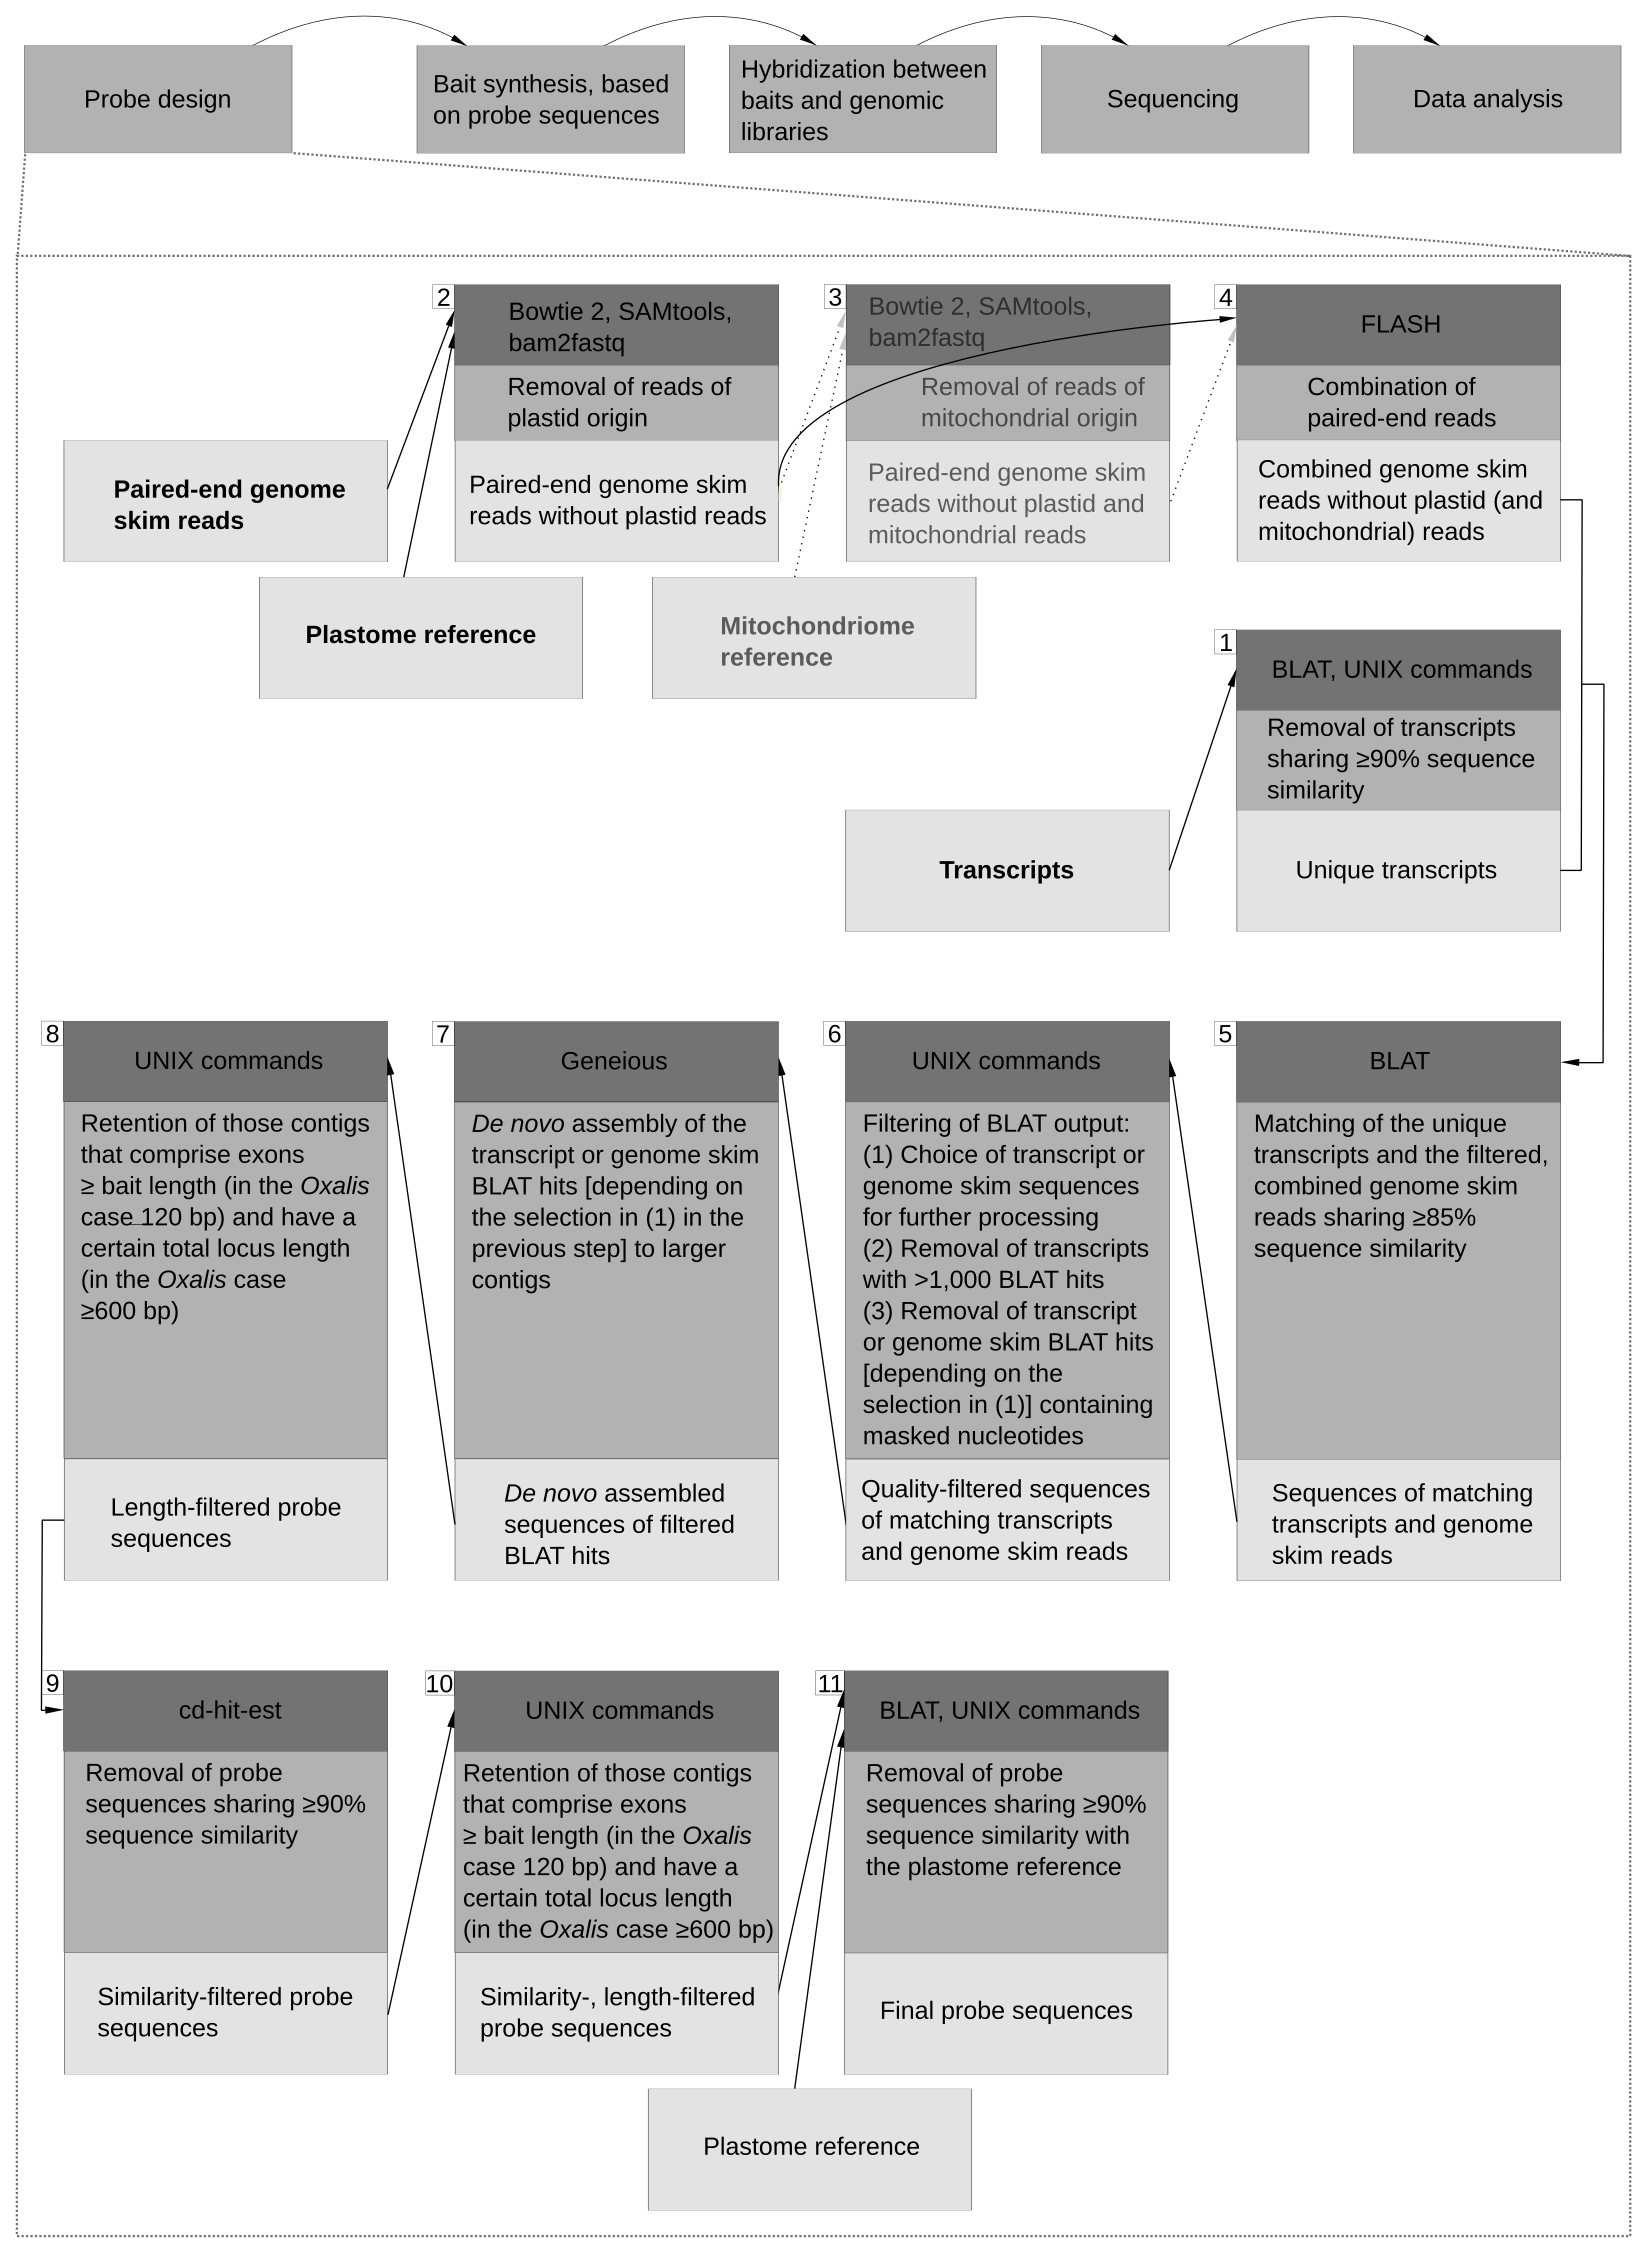
\includegraphics[width=15cm]{pipeline_workflow_grayscale.png}
\caption[Workflow of the probe design script Sondovač]{Workflow of the probe design script Sondovač. An overview on the main steps of Hyb-Seq are given in the top part of the figure; probe design is the first one. Each step of Sondovač is numbered and illustrated by three boxes each: Software is highlighted in dark gray, a summary of each step is given in medium gray, and input/output of each step is depicted in light gray. Optional removal of reads of mitochondrial origin from the genome skim data is marked by decoloration of the text. The required input files of Sondovač are highlighted in bold. The direction of the workflow is indicated by arrows.}
\label{pipeline-workflow}
\end{figure}

For comprehension improvement the steps of Sondovač are consecutively numbered. Sondovač has three parts: two script parts and an intermediate part using Geneious. The workflow is as follows:

\begin{enumerate}[label=\textbf{\Alph*.}]
  \label{pipeline-overview}
  \item \texttt{sondovac$\_$part$\_$a.sh}: Covers steps 1 to 6.
    \begin{enumerate}[label=\textbf{\arabic*.}]
      \item Removal of transcripts sharing $\geq$90\% sequence similarity.
      \item Removal of reads of plastid origin.
      \item Removal of reads of mitochondrial origin (optional).
      \item Combination of paired-end reads.
      \item Matching of the unique transcripts and the filtered, combined genome skim reads sharing $\geq$85\% sequence similarity.
      \item Filtering of BLAT output:
	\begin{enumerate}[label=\textbf{6.\arabic*.}]
	\item Choice of transcript or genome skim sequences for further processing.
	\item Removal of transcripts with $>$1000 BLAT hits.
	\item Removal of transcript or genome skim BLAT hits [depending on the selection in (6.1)] containing masked nucleotides.
	\end{enumerate}
    \end{enumerate}

  Input files for \texttt{sondovac$\_$part$\_$a.sh} are FASTA transcriptome data, FASTQ paired-end genome skim reads and a plastome (and possible as well mitochondriome) reference. The input file for Geneious is the output of \texttt{sondovac$\_$part$\_$a.sh}.

  \item Geneious: Covers step 7 (see below and PDF manual).
    \begin{enumerate}[label=\textbf{\arabic*.}, resume]
    \item De novo assembly of the transcript or genome skim BLAT hits [depending on the selection in (6.1)] to larger contigs. Note you need a copy of Geneious for this step.
    \end{enumerate}

  The output files of Geneious are input files for \texttt{sondovac$\_$part$\_$b.sh}.

  \item \texttt{sondovac$\_$part$\_$b.sh}: Covers steps 8 to 11.
    \begin{enumerate}[label=\textbf{\arabic*.}, resume]
      \item Retention of those contigs that comprise exons $\geq$ bait length and have a certain total locus length.
      \item Removal of probe sequences sharing $\geq$90\% sequence similarity.
      \item Retention of those contigs that comprise exons $\geq$ bait length and have a certain total locus length.
      \item Removal of probe sequences sharing $\geq$90\% sequence similarity with the plastome reference.
    \end{enumerate}

  The output file of \texttt{sondovac$\_$part$\_$b.sh} is the final list of probes.

\end{enumerate}

\section{Installation of Sondovač}
\label{install}

Sondovač is simple BASH script, but it requires some software. The script will check for presence of all required software and if needed, it will offer installation. The most easy way is just to launch the script (see chapter \ref{script-start} at page \pageref{script-start}) and yet yourselves to be guided through whole needed process.

\subsection{Requirements to run Sondovač}

Sondovač is currently tested on the Linux distributions Ubuntu and openSUSE. Testing on Mac OS X and other major Linux distributions is on the way and full support will be added soon. Thank you for patience and reporting\footnote{You can report any problems at \href{https://github.com/V-Z/sondovac/issues}{https://github.com/V-Z/sondovac/issues}. We will try to help you.} any problems and wishes.

In order to run Sondovač you need a UNIX-based operating system (preferably Linux or Mac OS X) equipped with BASH or compatible shell interpreter (this should be by default available for any Linux distribution, Mac OS X and any other UNIX-based operating system like Solaris, BSD and its variants etc). You should use the current operating system version supported by upstream. Otherwise we will not be able to help you in case of problems. Older operating systems can have different versions of shell and system libraries, which can cause various problems and incompatibilities.

Sondovač is using several scientific software packages (namely bam2fastq, BLAT, Bowtie2, CD-HIT, FASTX toolkit, FLASH, htsjdk, libgtextutils, Picard and SAMtools -- see required versions and links below), and basic UNIX tools. Sondovač will check if those programs are installed -- available in the PATH (i.e. if the shell application can locate and launch respective binaries). If you have those packages installed (in current versions), ensure their binaries are in PATH. This should not be a problem for basic tools available in any UNIX-based operating system, as basic installation usually contains all needed tools. If you are lacking some of the required tools, the script will notify you, and you will have to install them manually. If this will be needed, check the documentation for your operating system.

If required scientific programs are not installed, Sondovač will offer you installation. You can use precompiled binaries available together with the script or (sometimes) from the web. This is the recommended way. In case you would like to compile required software yourselves, the script will guide you through this process. Anyway, it is recommended only for advanced users, as compilation might sometimes be very tricky. It is currently fully implemented only for the Linux distributions Ubuntu and openSUSE. Support for other Linux distributions and Mac OS X will be added soon. For compilation you need Apache Ant, GNU G++, GNU GCC, GIT, Java, libpng developmental files and zlib developmental files. Ensure you have those tools available -- they should be readily available for any UNIX-based operating system.

\subsection{First launch of Sondovač}
\label{script-start}

Download the latest version from \href{https://github.com/V-Z/sondovac/releases/}{https://github.com/V-Z/sondovac/releases/} and unpack the archive. You can run Sondovač from any directory. In command line navigate to the directory with the unpacked Sondovač files (see Figure~\ref{terminal}):

\begin{bashcode}
  cd /path/to/directory_with_sondovac
\end{bashcode}

and start it by

\begin{bashcode}
  ./sondovac_part_a.sh -h
\end{bashcode}

to see basic usage instructions. See chapter~\ref{script-usage} at page~\pageref{script-usage} for more information.

\begin{figure}[htbp]
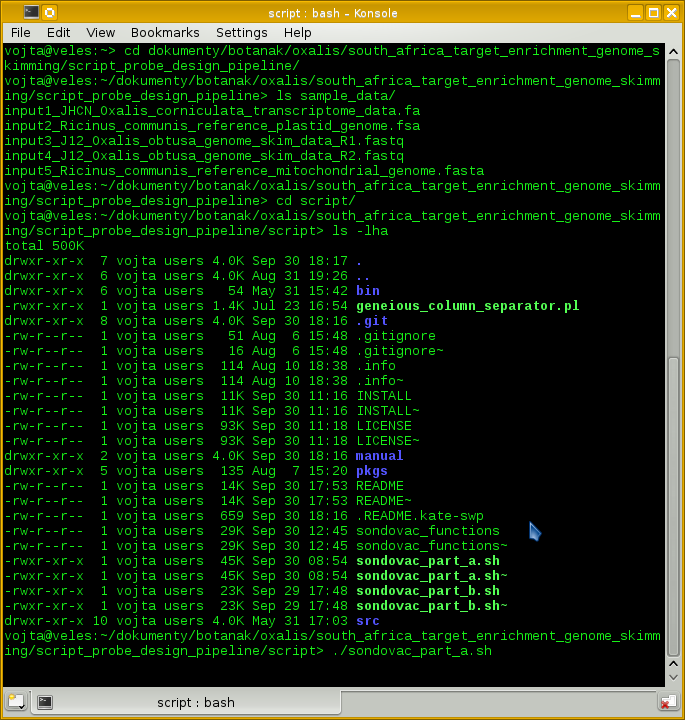
\includegraphics[width=\textwidth]{terminal.png}
\caption[Starting terminal and navigating to Sondovač]{Starting terminal and navigating to Sondovač. First look at the terminal (command-line, shell) window, navigation to directory with Sondovač (using command \texttt{cd}), listing directory content (command \texttt{ls}) and preparing to launch Sondovač (\texttt{./sondovac$\_$part$\_$a.sh}).}
\label{terminal}
\end{figure}

\subsubsection{Examples (see further for explanation of command line parameters)}

Basic and the most simple usage (running in interactive mode, see chapter~\ref{script-usage} at page~\pageref{script-usage}):

\begin{bashcode}
  ./sondovac_part_a.sh -i
\end{bashcode}

Specify some of required input files, otherwise run interactively:

\begin{bashcode}
  ./sondovac_part_a.sh -i -f input.fa -t reads1.fastq -q reads2.fastq
\end{bashcode}

Running in non-interactive automated way (parameter "\texttt{-n}", see chapter~\ref{script-usage} at page~\pageref{script-usage}) with 
example data downloaded from \href{https://github.com/V-Z/sondovac/wiki/Sample-data}{https://github.com/V-Z/sondovac/wiki/Sample-data}:

\begin{bashcode}
  ./sondovac_part_a.sh -f input1_JHCN_Oxalis_corniculata_transcriptome_data.fa \
   -c input2_Ricinus_communis_reference_plastid_genome.fsa -m \
   input5_Ricinus_communis_reference_mitochondrial_genome.fasta -t \
   input3_J12_Oxalis_obtusa_genome_skim_data_R1.fastq -q \
   input4_J12_Oxalis_obtusa_genome_skim_data_R2.fastq -n
\end{bashcode}

Modify parameter "\texttt{-a}", otherwise run interactively:

\begin{bashcode}
  ./sondovac_part_a.sh -i -a 300
\end{bashcode}

Run in non-interactive mode (parameter "\texttt{-n}", see chapter~\ref{script-usage} at page~\pageref{script-usage}) -- in such case user must specify all required input files (parameters "\texttt{-f}", "\texttt{-c}", "\texttt{-m}", "\texttt{-t}" and "\texttt{-q}"). Moreover, parameter "\texttt{-y}" is modified:

\begin{bashcode}
  ./sondovac_part_a.sh -n -f input.fa -c referencecp.fasta \
   -m referencemt.fsa -t reads1.fastq -q reads2.fastq -y 90
\end{bashcode}

Modifying parameter "\texttt{-s}". Note interactive mode "\texttt{-i}" is implicit and does not need to be specified explicitly:

\begin{bashcode}
  ./sondovac_part_a.sh -s 950
\end{bashcode}

\subsection{Help for usage of terminal}

If you are not familiar with the usage of command line, see some basic tutorial first. You can try some of those:

\begin{itemize}
\item \href{https://activedoc.opensuse.org/book/opensuse-start-up/chapter-17-shell-basics}{https://activedoc.opensuse.org/book/opensuse-start-up/chapter-17-shell-basics}
\item \href{https://help.ubuntu.com/community/UsingTheTerminal}{https://help.ubuntu.com/community/UsingTheTerminal}
\item \href{https://www.gnu.org/software/bash/manual/}{https://www.gnu.org/software/bash/manual/} (advanced -- full reference manual)
\item \href{http://ubuntuguide.org/}{http://ubuntuguide.org/}
\item \href{https://www.debian.org/doc/manuals/debian-reference/ch01.en.html}{https://www.debian.org/doc/manuals/debian-reference/ch01.en.html}
\item \href{https://trapa.cz/en/course-linux-command-line-2015}{https://trapa.cz/en/course-linux-command-line-2015}
\item \href{https://docs.fedoraproject.org/en-US/Fedora/22/html/System_Administrators_Guide}{https://docs.fedoraproject.org/en-US/Fedora/22/html/System$\_$Administrators$\_$Guide}
\end{itemize}

\subsection{Geneious}

For the part (2) user must have Geneious. Geneious is a DNA alignment, assembly, and analysis software and one of the most common software platforms used in genomics. It is utilized for de novo assembly in Sondovač. We plan to replace it by some free open-source command line tool in some future release of Sondovač. Visit \href{http://www.geneious.com/}{http://www.geneious.com/} for download, purchase, installation and usage of Geneious. It is very feature-rich application.

Geneious was tested with versions 6, 7 and 8.

Import output file of part A of the script (\texttt{sondovac$\_$part$\_$a.sh}): go to menu \textbf{File | Import | From File\ldots} This file is named as:\\YourInputFile$\_$blat$\_$unique$\_$transcripts$\_$versus$\_$genome$\_$skim$\_$data-no$\_$missing$\_$fin.fsa

Select the file and go to menu \textbf{Tools | Align / Assemble | De Novo Assemble}. In \textbf{Data} frame select \textbf{Assembe by 1st (\ldots) Underscore}. In \textbf{Method} frame select \textbf{Geneious Assembler} (if you don't have other assemblers, this option might be missing) and \textbf{Medium Sensitivity / Fast Sensitivity}

In \textbf{Results} frame check \textbf{Save assembly report}, \textbf{Save list of unused reads}, \textbf{Save in sub-folder}, \textbf{Save contigs} (do not check \textbf{Maximum}) and \textbf{Save consensus sequences}. Do not trim. Otherwise keep defaults. Run it. Geneious may warn about possible hanging because of big file. Do not use Geneious for other tasks during the assembly. Running may take long time.

Select all resulting contigs (typically named \textbf{* Contig \#}) and export them (go to menu \textbf{File | Export | Selected Documents\ldots}) as \textbf{Tab-separated table values (*.tsv)}. Save following columns (Hold \texttt{Ctrl} key to mark more fields): \textbf{\# Sequences}, \textbf{\% Pairwise Identity}, \textbf{Description}, \textbf{Mean Coverage}, \textbf{Name} and \textbf{Sequence Length}. If this option would be inaccessible for you, export all columns.

Select items \textbf{Consensus Sequences} and \textbf{Unused Reads} and export them as one \textbf{FASTA}. Go to menu \textbf{File | Export | Selected Documents\ldots} and choose \textbf{FASTA file type}.

Use exported files from Geneious as input for part B of the script (\texttt{sondovac$\_$part$\_$b.sh}).

\subsection{Software used by Sondovač}

Table~\ref{software-links} lists all software used by Sondovač, including minimal required versions and homepages. As soon as you have recent version of your operating system and you are using automated way of installation of additional software offered by Sondovač, you do not have to worry about this. In case you installed some of required scientific packages manually, ensure you have required minimal version. Following list refers papers and web resources describing methods used by software used by Sondovač:

\begin{table}[htb]
\caption[Required software, its versions and homepages.]{Required software, its versions and homepages. "X" denotes any subversion of particular lineage and "v. $>$" denotes any version higher then noted. Generally, any current version should usually be fine.}
\begin{tabular}{lll}
\textbf{Software} & \textbf{Version} & \textbf{Homepage}\\
Apache Ant & 1.9.X & \href{https://ant.apache.org/}{https://ant.apache.org/}\\
bam2fastq & 1.1.0 & \href{http://gsl.hudsonalpha.org/information/software/bam2fastq}{http://gsl.hudsonalpha.org/information/software/bam2fastq}\\
BASH & v. > 3 & \href{https://gnu.org/software/bash/bash.html}{https://gnu.org/software/bash/bash.html}\\
BLAT & v.36 & \href{http://genome.ucsc.edu/FAQ/FAQblat.html}{http://genome.ucsc.edu/FAQ/FAQblat.html}\\
Bowtie2 & 2.2.6 & \href{http://bowtie-bio.sourceforge.net/bowtie2/index.shtml}{http://bowtie-bio.sourceforge.net/bowtie2/index.shtml}\\
CD-HIT & 4.6 & \href{http://weizhongli-lab.org/cd-hit/}{http://weizhongli-lab.org/cd-hit/}\\
FASTX, libgtextutils & 0.0.13 & \href{http://hannonlab.cshl.edu/fastx_toolkit/}{http://hannonlab.cshl.edu/fastx$\_$toolkit/}\\
FLASH & 1.2.11 & \href{http://sourceforge.net/projects/flashpage/}{http://sourceforge.net/projects/flashpage/}\\
G++, GCC & v. > 4.2 & \href{http://gcc.gnu.org/}{http://gcc.gnu.org/}\\
Geneious & v. > 6.1 & \href{http://www.geneious.com/}{http://www.geneious.com/}\\
GIT & v. > 2.0 & \href{http://git-scm.com/}{http://git-scm.com/}\\
GNU core utils & 8.X & \href{https://gnu.org/software/coreutils/coreutils.html}{https://gnu.org/software/coreutils/coreutils.html}\\
Java/OpenJDK & v. > 7 & \href{https://www.java.com/}{https://www.java.com/}/\href{http://openjdk.java.net/}{http://openjdk.java.net/}\\
libpng & 1.6.X & \href{http://www.libpng.org/}{http://www.libpng.org/}\\
Picard & v. > 1.137 & \href{https://broadinstitute.github.io/picard/}{https://broadinstitute.github.io/picard/}\\
SAMtools, htsjdk & 1.2 & \href{http://www.htslib.org/}{http://www.htslib.org/}\\
Sondovač & 0.6 & \href{https://github.com/V-Z/sondovac/wiki}{https://github.com/V-Z/sondovac/wiki}\\
zlib & 1.2.8 & \href{http://zlib.net/}{http://zlib.net/}
\end{tabular}
\label{software-links}
\end{table}

\begin{description}
 \item[BLAT] Kent: BLAT -- the BLAST-like alignment tool, \href{http://genome.cshlp.org/content/12/4/656.short}{http://genome.cshlp.org/content/12/4/656.short}
 \item[Bowtie2] Langmead and Salzberg: Fast gapped-read alignment with Bowtie 2, \href{http://www.nature.com/nmeth/journal/v9/n4/full/nmeth.1923.html}{http://www.nature.com/nmeth/journal/v9/n4/full/nmeth.1923.html}
 \item[CD-HIT] There are several papers describing CD-HIT:
  \begin{itemize}
    \item Li et al: Clustering of highly homologous sequences to reduce the size of large protein databases, \href{http://bioinformatics.oxfordjournals.org/content/17/3/282.short}{http://bioinformatics.oxfordjournals.org/content/17/3/282.short}
    \item Li et al: Tolerating some redundancy significantly speeds up clustering of large protein databases, \href{http://bioinformatics.oxfordjournals.org/content/18/1/77.short}{http://bioinformatics.oxfordjournals.org/content/18/1/77.short}
    \item Li and Godzik: Cd-hit: a fast program for clustering and comparing large sets of protein or nucleotide sequences, \href{http://bioinformatics.oxfordjournals.org/content/22/13/1658.short}{http://bioinformatics.oxfordjournals.org/content/22/13/1658.short}
    \item Fu et al: CD-HIT: accelerated for clustering the next generation sequencing data, \href{http://bioinformatics.oxfordjournals.org/content/28/23/3150.short}{http://bioinformatics.oxfordjournals.org/content/28/23/3150.short}
    \item Huang et al: CD-HIT Suite: a web server for clustering and comparing biological sequences, \href{http://bioinformatics.oxfordjournals.org/content/26/5/680.short}{http://bioinformatics.oxfordjournals.org/content/26/5/680.short}
    \item Niu et al: Artificial and natural duplicates in pyrosequencing reads of metagenomic data, \href{http://www.biomedcentral.com/1471-2105/11/187}{http://www.biomedcentral.com/1471-2105/11/187}
    \item Li et al: Ultrafast clustering algorithms for metagenomic sequence analysis, \href{http://bib.oxfordjournals.org/content/13/6/656.abstract}{http://bib.oxfordjournals.org/content/13/6/656.abstract}
   \end{itemize}
 \item[FASTX toolkit] Gordon and Hannon: FASTX-Toolkit. FASTQ/A short-reads pre-processing tools, \href{http://hannonlab.cshl.edu/fastx_toolkit/}{http://hannonlab.cshl.edu/fastx$\_$toolkit/}
 \item[FLASH] Magoč and Salzberg: FLASH: fast length adjustment of short reads to improve genome assemblies, \href{http://bioinformatics.oxfordjournals.org/content/27/21/2957.abstract}{http://bioinformatics.oxfordjournals.org/content/27/21/2957.abstract}
 \item[SAMtools] There are several papers describing SAMtools:
  \begin{itemize}
   \item Li et al.: The Sequence alignment/map (SAM) format and SAMtools, \href{http://bioinformatics.oxfordjournals.org/content/25/16/2078.abstract}{http://bioinformatics.oxfordjournals.org/content/25/16/2078.abstract}
   \item Li: A statistical framework for SNP calling, mutation discovery, association mapping and population genetical parameter estimation from sequencing data, \href{http://bioinformatics.oxfordjournals.org/content/27/21/2987.abstract}{http://bioinformatics.oxfordjournals.org/content/27/21/2987.abstract}
   \item Li et al: Improving SNP discovery by base alignment quality, \href{http://bioinformatics.oxfordjournals.org/content/27/8/1157.short}{http://bioinformatics.oxfordjournals.org/content/27/8/1157.short}
  \end{itemize}
 \item[Sondovač] Schmickl et al
\end{description}

\subsection{Vocabulary}

\begin{description}
\item[Binary] An application in form understandable by the computer, but usually not transferable among operating systems and/or hardware platforms. Binaries in Windows usually have extension *.exe, in UNIX there use to be no extension.
\item[BASH] "The command line" -- fully featured programming scripting language accessible through terminal of any UNIX-based operating system (any Linux, Mac OS X, Solaris, any variant of BSD and more). BASH scripts usually have extension *.sh.
\item[BSD] Group of popular UNIX-based operating systems. See \href{https://en.wikipedia.org/wiki/Berkeley_Software_Distribution}{https://en.wikipedia.org/wiki/Berkeley$\_$Software$\_$Distribution}.
\item[compilation] "Translation" of software application from the source code (text readable by human programmer) into binary form launchable by the computer. It requires special tools, and it usually must be done for every operating system and hardware platform.
\item[Console] See "Shell".
\item[GNU] Major project providing free software widely used in many operating systems, see \href{https://gnu.org/}{https://gnu.org/}.
\item[Library] Pack of software tools and functions used by another applications.
\item[Linux] One of the most common variants of UNIX-based operating systems. Linux kernel is used by many developers, so that there are plenty of Linux distributions ("flavors") from various sources (e.g. Ubuntu and derivatives, openSUSE, SLE, Debian, Linux Mint, Fedora, Centos, RedHat etc.). They share many features although on the first look they can look differently. See \href{https://en.wikipedia.org/wiki/Linux}{https://en.wikipedia.org/wiki/Linux}.
\item[Mac OS X] Popular operating system produced by Apple. The system kernel is based on UNIX, see \href{https://www.apple.com/osx/}{https://www.apple.com/osx/}.
\item[openSUSE] Popular Linux distribution, see \href{https://www.opensuse.org/}{https://www.opensuse.org/}.
\item[Operating system] Basic system running on your computer -- typically MS Windows (not supported by Sondovač, although it might be working), Mac OS X or some Linux distribution (Ubuntu and derivatives, openSUSE, SLE, Debian, Linux Mint, Fedora, Centos, RedHat etc.).
\item[Parameter(s)] Option(s) passed to any function/command line application to modify its usage. Some can be required, some are optional and some can be used only in particular cases. In case of shell applications, parameters are usually given in way like "application -X", "application -\-parameter", "application -Param SomeValue" and so on. See manual for particular application (e.g. "man application"), in case of Sondovač see XXX. % Link to commands
\item[PATH] Directories in the computer where the system is looking for installed software (in a UNIX-based system you can view it by the command "\texttt{echo \$PATH}"). If you need to modify it manually, see the documentation for your operating system.
\item[Script] Software application. It requires an interpreter (application installed on the computer that is able to launch scripts written in a particular language), but the application itself is portable among operating systems and hardware architectures, and it is written in plain text, so that developers can easily modify it. Common examples are Python, Perl or BASH.
\item[Shell] "The command line" -- the interface to interact with software using commands typed into the terminal window (See Figure~\ref{terminal}).
\item[Solaris] Popular (mainly on servers) UNIX-based operating system, now developed by Oracle and including several independent clones. See \href{http://distrowatch.com/table.php?distribution=solaris}{http://distrowatch.com/table.php?distribution=solaris}.
\item[Terminal] see "Shell".
\item[Ubuntu] Popular Linux distribution, see \href{http://www.ubuntu.com/}{http://www.ubuntu.com/}.
\item[Upstream] Developers usually support (e.g. by fixing of bugs) only newer versions of an application. If you use an older version and you encounter problems, no one will probably help you. Moreover, using old versions of software can be a security risk because of security issues fixed in newer versions.
\item[UNIX (UNIX-like, UN*X, *nix,~\ldots)] Family of operating systems sharing the same logic, software architecture and plenty of tools. See \href{https://en.wikipedia.org/wiki/Unix-like}{https://en.wikipedia.org/wiki/Unix-like} for details.
\end{description}

\section{Usage of Sondovač}
\label{script-usage}

\subsection{Command line parameters}

Sondovač has some parameters useful especially for advanced users, on remote servers, for repeated analysis and so on. We recommend to start with basic interactive usage -- script will ask for input files and when needed also for installation of additional software.

\begin{bashcode}
  # Go to directory with unpacked Sondovač (in terminal):
  cd /path/to/directory_with_sondovac
  # Run sondovac_part_a.sh in basic interactive mode:
  ./sondovac_part_a.sh -i
  # Then run Geneious and continue with sondovac_part_b.sh:
  ./sondovac_part_b.sh -i
\end{bashcode}

\subsubsection{General parameters}

Shared by \texttt{sondovac$\_$part$\_$a.sh} as well as \texttt{sondovac$\_$part$\_$b.sh}.

\begin{description}
  \item[\texttt{-h}, \texttt{-v}] Print help message and exit.
  \item[\texttt{-u}] Check for updates. If there is newer version of Sondovač available on \href{https://github.com/V-Z/sondovac/releases/}{https://github.com/V-Z/sondovac/releases/} download of newer version will be offered to the user.
  \item[\texttt{-l}] Display LICENSE for license information (this script is licensed under GNU GPL v.3, other software under variable licenses). Exit viewing by pressing the \texttt{Q} key.
  \item[\texttt{-r}] Display README for detailed usage instructions. Exit viewing by pressing the \texttt{Q} key.
  \item[\texttt{-p}] Display INSTALL for detailed installation instructions. Exit viewing by pressing the \texttt{Q} key. See also page~\pageref{install}.
  \item[\texttt{-e}] Display detailed citation information and exit.
  \item[\texttt{-i}] Running in interactive mode -- script will on-demand ask for required input files, installation of missing software etc. This is recommended default value (the script runs interactively without explicit using option \texttt{-n}).
  \item[\texttt{-n}] Running in non-interactive mode. User must provide at least required input files (see below). You can use only one of parameters \texttt{-i} or \texttt{-n} (not both of them). If script fails to find some of required software packages, it will exit. This is recommended for batch or repeated analysis, on remote servers and for more advanced users. User must be sure that all required software is installed (see page~\pageref{install}).
\end{description}

\subsubsection{Input files}

Those parameters are required when running in non-interactive mode. The parameters are optional in default interactive mode. Please, use file names without spaces and without special characters.

\begin{description}
\item[\texttt{-f FILE}] Transcriptome input file in FASTA format.
  \begin{itemize}
    \item \texttt{sondovac$\_$part$\_$a.sh}
  \end{itemize}
\item[\texttt{-c FILE}] Plastome reference sequence input file in FASTA format.
  \begin{itemize}
    \item \texttt{sondovac$\_$part$\_$a.sh}, \texttt{sondovac$\_$part$\_$b.sh}
    \item Plastome reference sequences from taxa up to the same order of the studied plant group are suitable. See Straub et al. 2012, \href{http://www.amjbot.org/content/99/2/349.short}{http://www.amjbot.org/content/99/2/349.short}.
  \end{itemize}
\item[\texttt{-m FILE}] Mitochondriome reference sequence input file in FASTA format (optional).
  \begin{itemize}
    \item \texttt{sondovac$\_$part$\_$a.sh}
    \item This step is facultative, as plant mitochondrial genomes have largely variable sizes and high rearrangement rates.
  \end{itemize}
\item[\texttt{-t FILE}] Paired-end genome skim input file in FASTQ format (first file).
  \begin{itemize}
    \item \texttt{sondovac$\_$part$\_$a.sh}
  \end{itemize}
\item[\texttt{-q FILE}] Paired-end genome skim input file in FASTQ format (second file).
  \begin{itemize}
    \item \texttt{sondovac$\_$part$\_$a.sh}
  \end{itemize}
\item[\texttt{-x FILE}] Input file in TSV format (output of Geneious assembly).
  \begin{itemize}
    \item \texttt{sondovac$\_$part$\_$b.sh}
  \end{itemize}
\item[\texttt{-z FILE}] Input file in FASTA format (output of Geneious assembly).
  \begin{itemize}
    \item \texttt{sondovac$\_$part$\_$b.sh}
  \end{itemize}
\end{description}

\subsubsection{Optional parameters}

See page~\pageref{pipeline-overview} and Figure~\ref{pipeline-workflow} for steps referred here. If those parameters are not provided, default values are used and it is not possible to change them any time later (not even in interactive mode).

\begin{description}
\item[\texttt{-a \#\#\#}] Read length of paired-end genome skim reads (parameter -M of FLASH, see its manual for details).
  \begin{itemize}
    \item Step 4 of Sondovač, \texttt{sondovac$\_$part$\_$a.sh}.
    \item Ensure to use a certain insert size of the genome skim genomic library in combination with an appropriate read length for sequencing in order to enable merging of the paired-end genome skim reads.
    \item DEFAULT: 250
    \item OPTIONS: 125, 150, 250, 300
  \end{itemize}
\item[\texttt{-y \#\#}] Sequence similiarity between unique transcripts and the filtered, combined genome skim reads (parameter -minIdentity of BLAT, see its manual for details).
  \begin{itemize}
    \item Step 5 of Sondovač, \texttt{sondovac$\_$part$\_$a.sh}.
    \item Consider the trade-off between probe specificity and number of remaining matching sequences for probe design. Sequence similarity is in percent.
    \item DEFAULT: 85
    \item OPTIONS: Integer ranging from 70 to 100
  \end{itemize}
\item[\texttt{-s \#\#\#\#}] Number of BLAT hits per transcript when matching unique transcripts and the filtered, combined genome skim reads.
  \begin{itemize}
    \item Step 6.2 of Sondovač, \texttt{sondovac$\_$part$\_$a.sh}.
    \item Transcripts with a high number of BLAT hits, indicating repetitive elements, need to be removed from the putative probe sequences.
    \item DEFAULT: 1000
    \item OPTIONS: Integer ranging from 100 to 10000
  \end{itemize}
\item[\texttt{-b \#\#\#}] Minimum exon (bait) length.
  \begin{itemize}
    \item Steps 8 and 10 of Sondovač, \texttt{sondovac$\_$part$\_$b.sh}.
    \item The minimum exon length should not fall below the bait length in order to facilitate specific binding between genomic libraries and baits during hybridization.
    \item DEFAULT: 120 (optimal length for phylogeny).
    \item OPTIONS: Integer ranging from 120 to 200
  \end{itemize}
\item[\texttt{-d 0.\#\#}] Sequence similarity between probe sequences (parameter -c of cd-hit-est, see its manual for details).
  \begin{itemize}
    \item Step 9 of Sondovač, \texttt{sondovac$\_$part$\_$b.sh}.
    \item Too similar probe sequences will interact with each other during hybridization and thereby reduce enrichment efficiency.
    \item DEFAULT: 0.9 (highly recommended).
    \item OPTIONS: Decimal ranging from 0.85 to 0.95
  \end{itemize}
\end{description}

\subsection{Input and output files}

XXX

\section{Questions not covered here, reporting bugs and wishes}

If you have any question or you encounter some problem, please, see \href{https://github.com/V-Z/sondovac/issues}{https://github.com/V-Z/sondovac/issues} and feel free to ask any question and/or express any wish. The authors will do their best to help you.

\section{Licenses}

The set of BASH scripts Sondovač is licensed under GNU General Public License version 3. List of licenses of included software is in Table~\ref{software-lic} (see full texts below). License of BLAT does not allow redistribution, so that this software is not included and the software is downloaded on the fly. Script is also using software included in GNU core utilities (basic tools available in any UNIX-based system), see \href{https://www.gnu.org/software/coreutils/}{https://www.gnu.org/software/coreutils/} for details.

\begin{table}[htb]
\caption[List of software and licenses]{List of software, licenses and links to license details}
\begin{tabular}{lll}
\textbf{Software} & \textbf{License} & \textbf{License details}\\
Sondovač & GNU GPL v. 3 & \href{https://gnu.org/licenses/gpl.html}{https://gnu.org/licenses/gpl.html}\\
Bowtie2 & GNU GPL v. 3 & \href{https://gnu.org/licenses/gpl.html}{https://gnu.org/licenses/gpl.html}\\
SAMtools & MIT/Expat Lic. & \href{https://en.wikipedia.org/wiki/MIT_License}{https://en.wikipedia.org/wiki/MIT$\_$License}\\
bam2fastq & Apache Lic. 2.0 & \href{https://apache.org/licenses/LICENSE-2.0.html}{https://apache.org/licenses/LICENSE-2.0.html}\\
Picard & MIT License & \href{https://en.wikipedia.org/wiki/MIT_License}{https://en.wikipedia.org/wiki/MIT$\_$License}\\
FLASh & GNU GPL v. 3 & \href{https://gnu.org/licenses/gpl.html}{https://gnu.org/licenses/gpl.html}\\
CD-HIT & GNU GPL v. 2 & \href{https://gnu.org/licenses/old-licenses/gpl-2.0.html}{https://gnu.org/licenses/old-licenses/gpl-2.0.html}\\
FASTX & GNU Affero GPL & \href{https://gnu.org/licenses/agpl.html}{https://gnu.org/licenses/agpl.html}
\end{tabular}
\label{software-lic}
\end{table}

\subsection{GNU GENERAL PUBLIC LICENSE, Version 3, 29 June 2007}

Copyright © 2007 Free Software Foundation, Inc. \href{http://fsf.org/}{http://fsf.org/}

Everyone is permitted to copy and distribute verbatim copies of this license document, but changing it is not allowed.

\subsubsection{Preamble}

The GNU General Public License is a free, copyleft license for software and other kinds of works.

The licenses for most software and other practical works are designed to take away your freedom to share and change the works. By contrast, the GNU General Public License is intended to guarantee your freedom to share and change all versions of a program--to make sure it remains free software for all its users. We, the Free Software Foundation, use the GNU General Public License for most of our software; it applies also to any other work released this way by its authors. You can apply it to your programs, too.

When we speak of free software, we are referring to freedom, not price. Our General Public Licenses are designed to make sure that you have the freedom to distribute copies of free software (and charge for them if you wish), that you receive source code or can get it if you want it, that you can change the software or use pieces of it in new free programs, and that you know you can do these things.

To protect your rights, we need to prevent others from denying you these rights or asking you to surrender the rights. Therefore, you have certain responsibilities if you distribute copies of the software, or if you modify it: responsibilities to respect the freedom of others.

For example, if you distribute copies of such a program, whether gratis or for a fee, you must pass on to the recipients the same freedoms that you received. You must make sure that they, too, receive or can get the source code. And you must show them these terms so they know their rights.

Developers that use the GNU GPL protect your rights with two steps: (1) assert copyright on the software, and (2) offer you this License giving you legal permission to copy, distribute and/or modify it.

For the developers' and authors' protection, the GPL clearly explains that there is no warranty for this free software. For both users' and authors' sake, the GPL requires that modified versions be marked as changed, so that their problems will not be attributed erroneously to authors of previous versions.

Some devices are designed to deny users access to install or run modified versions of the software inside them, although the manufacturer can do so. This is fundamentally incompatible with the aim of protecting users' freedom to change the software. The systematic pattern of such abuse occurs in the area of products for individuals to use, which is precisely where it is most unacceptable. Therefore, we have designed this version of the GPL to prohibit the practice for those products. If such problems arise substantially in other domains, we stand ready to extend this provision to those domains in future versions of the GPL, as needed to protect the freedom of users.

Finally, every program is threatened constantly by software patents. States should not allow patents to restrict development and use of software on general-purpose computers, but in those that do, we wish to avoid the special danger that patents applied to a free program could make it effectively proprietary. To prevent this, the GPL assures that patents cannot be used to render the program non-free.

The precise terms and conditions for copying, distribution and modification follow.

\subsubsection{TERMS AND CONDITIONS}

\subsubsection{0. Definitions}

“This License” refers to version 3 of the GNU General Public License.

“Copyright” also means copyright-like laws that apply to other kinds of works, such as semiconductor masks.

“The Program” refers to any copyrightable work licensed under this License. Each licensee is addressed as “you”. “Licensees” and “recipients” may be individuals or organizations.

To “modify” a work means to copy from or adapt all or part of the work in a fashion requiring copyright permission, other than the making of an exact copy. The resulting work is called a “modified version” of the earlier work or a work “based on” the earlier work.

A “covered work” means either the unmodified Program or a work based on the Program.

To “propagate” a work means to do anything with it that, without permission, would make you directly or secondarily liable for infringement under applicable copyright law, except executing it on a computer or modifying a private copy. Propagation includes copying, distribution (with or without modification), making available to the public, and in some countries other activities as well.

To “convey” a work means any kind of propagation that enables other parties to make or receive copies. Mere interaction with a user through a computer network, with no transfer of a copy, is not conveying.

An interactive user interface displays “Appropriate Legal Notices” to the extent that it includes a convenient and prominently visible feature that (1) displays an appropriate copyright notice, and (2) tells the user that there is no warranty for the work (except to the extent that warranties are provided), that licensees may convey the work under this License, and how to view a copy of this License. If the interface presents a list of user commands or options, such as a menu, a prominent item in the list meets this criterion.

\subsubsection{1. Source Code}

The “source code” for a work means the preferred form of the work for making modifications to it. “Object code” means any non-source form of a work.

A “Standard Interface” means an interface that either is an official standard defined by a recognized standards body, or, in the case of interfaces specified for a particular programming language, one that is widely used among developers working in that language.

The “System Libraries” of an executable work include anything, other than the work as a whole, that (a) is included in the normal form of packaging a Major Component, but which is not part of that Major Component, and (b) serves only to enable use of the work with that Major Component, or to implement a Standard Interface for which an implementation is available to the public in source code form. A “Major Component”, in this context, means a major essential component (kernel, window system, and so on) of the specific operating system (if any) on which the executable work runs, or a compiler used to produce the work, or an object code interpreter used to run it.

The “Corresponding Source” for a work in object code form means all the source code needed to generate, install, and (for an executable work) run the object code and to modify the work, including scripts to control those activities. However, it does not include the work's System Libraries, or general-purpose tools or generally available free programs which are used unmodified in performing those activities but which are not part of the work. For example, Corresponding Source includes interface definition files associated with source files for the work, and the source code for shared libraries and dynamically linked subprograms that the work is specifically designed to require, such as by intimate data communication or control flow between those subprograms and other parts of the work.

The Corresponding Source need not include anything that users can regenerate automatically from other parts of the Corresponding Source.

The Corresponding Source for a work in source code form is that same work.

\subsubsection{2. Basic Permissions}

All rights granted under this License are granted for the term of copyright on the Program, and are irrevocable provided the stated conditions are met. This License explicitly affirms your unlimited permission to run the unmodified Program. The output from running a covered work is covered by this License only if the output, given its content, constitutes a covered work. This License acknowledges your rights of fair use or other equivalent, as provided by copyright law.

You may make, run and propagate covered works that you do not convey, without conditions so long as your license otherwise remains in force. You may convey covered works to others for the sole purpose of having them make modifications exclusively for you, or provide you with facilities for running those works, provided that you comply with the terms of this License in conveying all material for which you do not control copyright. Those thus making or running the covered works for you must do so exclusively on your behalf, under your direction and control, on terms that prohibit them from making any copies of your copyrighted material outside their relationship with you.

Conveying under any other circumstances is permitted solely under the conditions stated below. Sublicensing is not allowed; section 10 makes it unnecessary.

\subsubsection{3. Protecting Users' Legal Rights From Anti-Circumvention Law}

No covered work shall be deemed part of an effective technological measure under any applicable law fulfilling obligations under article 11 of the WIPO copyright treaty adopted on 20 December 1996, or similar laws prohibiting or restricting circumvention of such measures.

When you convey a covered work, you waive any legal power to forbid circumvention of technological measures to the extent such circumvention is effected by exercising rights under this License with respect to the covered work, and you disclaim any intention to limit operation or modification of the work as a means of enforcing, against the work's users, your or third parties' legal rights to forbid circumvention of technological measures.

\subsubsection{4. Conveying Verbatim Copies}

You may convey verbatim copies of the Program's source code as you receive it, in any medium, provided that you conspicuously and appropriately publish on each copy an appropriate copyright notice; keep intact all notices stating that this License and any non-permissive terms added in accord with section 7 apply to the code; keep intact all notices of the absence of any warranty; and give all recipients a copy of this License along with the Program.

You may charge any price or no price for each copy that you convey, and you may offer support or warranty protection for a fee.

\subsubsection{5. Conveying Modified Source Versions}

You may convey a work based on the Program, or the modifications to produce it from the Program, in the form of source code under the terms of section 4, provided that you also meet all of these conditions:

\begin{enumerate}[label=\Alph*)]
\item The work must carry prominent notices stating that you modified it, and giving a relevant date.
\item The work must carry prominent notices stating that it is released under this License and any conditions added under section 7. This requirement modifies the requirement in section 4 to “keep intact all notices”.
\item You must license the entire work, as a whole, under this License to anyone who comes into possession of a copy. This License will therefore apply, along with any applicable section 7 additional terms, to the whole of the work, and all its parts, regardless of how they are packaged. This License gives no permission to license the work in any other way, but it does not invalidate such permission if you have separately received it.
\item If the work has interactive user interfaces, each must display Appropriate Legal Notices; however, if the Program has interactive interfaces that do not display Appropriate Legal Notices, your work need not make them do so.
\end{enumerate}

A compilation of a covered work with other separate and independent works, which are not by their nature extensions of the covered work, and which are not combined with it such as to form a larger program, in or on a volume of a storage or distribution medium, is called an “aggregate” if the compilation and its resulting copyright are not used to limit the access or legal rights of the compilation's users beyond what the individual works permit. Inclusion of a covered work in an aggregate does not cause this License to apply to the other parts of the aggregate.

\subsubsection{6. Conveying Non-Source Forms}

You may convey a covered work in object code form under the terms of sections 4 and 5, provided that you also convey the machine-readable Corresponding Source under the terms of this License, in one of these ways:

\begin{enumerate}[label=\Alph*)]
\item Convey the object code in, or embodied in, a physical product (including a physical distribution medium), accompanied by the Corresponding Source fixed on a durable physical medium customarily used for software interchange.
\item Convey the object code in, or embodied in, a physical product (including a physical distribution medium), accompanied by a written offer, valid for at least three years and valid for as long as you offer spare parts or customer support for that product model, to give anyone who possesses the object code either (1) a copy of the Corresponding Source for all the software in the product that is covered by this License, on a durable physical medium customarily used for software interchange, for a price no more than your reasonable cost of physically performing this conveying of source, or (2) access to copy the Corresponding Source from a network server at no charge.
\item Convey individual copies of the object code with a copy of the written offer to provide the Corresponding Source. This alternative is allowed only occasionally and noncommercially, and only if you received the object code with such an offer, in accord with subsection 6b.
\item Convey the object code by offering access from a designated place (gratis or for a charge), and offer equivalent access to the Corresponding Source in the same way through the same place at no further charge. You need not require recipients to copy the Corresponding Source along with the object code. If the place to copy the object code is a network server, the Corresponding Source may be on a different server (operated by you or a third party) that supports equivalent copying facilities, provided you maintain clear directions next to the object code saying where to find the Corresponding Source. Regardless of what server hosts the Corresponding Source, you remain obligated to ensure that it is available for as long as needed to satisfy these requirements.
\item Convey the object code using peer-to-peer transmission, provided you inform other peers where the object code and Corresponding Source of the work are being offered to the general public at no charge under subsection 6d.
\end{enumerate}

A separable portion of the object code, whose source code is excluded from the Corresponding Source as a System Library, need not be included in conveying the object code work.

A “User Product” is either (1) a “consumer product”, which means any tangible personal property which is normally used for personal, family, or household purposes, or (2) anything designed or sold for incorporation into a dwelling. In determining whether a product is a consumer product, doubtful cases shall be resolved in favor of coverage. For a particular product received by a particular user, “normally used” refers to a typical or common use of that class of product, regardless of the status of the particular user or of the way in which the particular user actually uses, or expects or is expected to use, the product. A product is a consumer product regardless of whether the product has substantial commercial, industrial or non-consumer uses, unless such uses represent the only significant mode of use of the product.

“Installation Information” for a User Product means any methods, procedures, authorization keys, or other information required to install and execute modified versions of a covered work in that User Product from a modified version of its Corresponding Source. The information must suffice to ensure that the continued functioning of the modified object code is in no case prevented or interfered with solely because modification has been made.

If you convey an object code work under this section in, or with, or specifically for use in, a User Product, and the conveying occurs as part of a transaction in which the right of possession and use of the User Product is transferred to the recipient in perpetuity or for a fixed term (regardless of how the transaction is characterized), the Corresponding Source conveyed under this section must be accompanied by the Installation Information. But this requirement does not apply if neither you nor any third party retains the ability to install modified object code on the User Product (for example, the work has been installed in ROM).

The requirement to provide Installation Information does not include a requirement to continue to provide support service, warranty, or updates for a work that has been modified or installed by the recipient, or for the User Product in which it has been modified or installed. Access to a network may be denied when the modification itself materially and adversely affects the operation of the network or violates the rules and protocols for communication across the network.

Corresponding Source conveyed, and Installation Information provided, in accord with this section must be in a format that is publicly documented (and with an implementation available to the public in source code form), and must require no special password or key for unpacking, reading or copying.

\subsubsection{7. Additional Terms}

“Additional permissions” are terms that supplement the terms of this License by making exceptions from one or more of its conditions. Additional permissions that are applicable to the entire Program shall be treated as though they were included in this License, to the extent that they are valid under applicable law. If additional permissions apply only to part of the Program, that part may be used separately under those permissions, but the entire Program remains governed by this License without regard to the additional permissions.

When you convey a copy of a covered work, you may at your option remove any additional permissions from that copy, or from any part of it. (Additional permissions may be written to require their own removal in certain cases when you modify the work.) You may place additional permissions on material, added by you to a covered work, for which you have or can give appropriate copyright permission.

Notwithstanding any other provision of this License, for material you add to a covered work, you may (if authorized by the copyright holders of that material) supplement the terms of this License with terms:

\begin{enumerate}[label=\Alph*)]
\item Disclaiming warranty or limiting liability differently from the terms of sections 15 and 16 of this License; or
\item Requiring preservation of specified reasonable legal notices or author attributions in that material or in the Appropriate Legal Notices displayed by works containing it; or
\item Prohibiting misrepresentation of the origin of that material, or requiring that modified versions of such material be marked in reasonable ways as different from the original version; or
\item Limiting the use for publicity purposes of names of licensors or authors of the material; or
\item Declining to grant rights under trademark law for use of some trade names, trademarks, or service marks; or 
\item Requiring indemnification of licensors and authors of that material by anyone who conveys the material (or modified versions of it) with contractual assumptions of liability to the recipient, for any liability that these contractual assumptions directly impose on those licensors and authors.
\end{enumerate}

All other non-permissive additional terms are considered “further restrictions” within the meaning of section 10. If the Program as you received it, or any part of it, contains a notice stating that it is governed by this License along with a term that is a further restriction, you may remove that term. If a license document contains a further restriction but permits relicensing or conveying under this License, you may add to a covered work material governed by the terms of that license document, provided that the further restriction does not survive such relicensing or conveying.

If you add terms to a covered work in accord with this section, you must place, in the relevant source files, a statement of the additional terms that apply to those files, or a notice indicating where to find the applicable terms.

Additional terms, permissive or non-permissive, may be stated in the form of a separately written license, or stated as exceptions; the above requirements apply either way.

\subsubsection{8. Termination}

You may not propagate or modify a covered work except as expressly provided under this License. Any attempt otherwise to propagate or modify it is void, and will automatically terminate your rights under this License (including any patent licenses granted under the third paragraph of section 11).

However, if you cease all violation of this License, then your license from a particular copyright holder is reinstated (a) provisionally, unless and until the copyright holder explicitly and finally terminates your license, and (b) permanently, if the copyright holder fails to notify you of the violation by some reasonable means prior to 60 days after the cessation.

Moreover, your license from a particular copyright holder is reinstated permanently if the copyright holder notifies you of the violation by some reasonable means, this is the first time you have received notice of violation of this License (for any work) from that copyright holder, and you cure the violation prior to 30 days after your receipt of the notice.

Termination of your rights under this section does not terminate the licenses of parties who have received copies or rights from you under this License. If your rights have been terminated and not permanently reinstated, you do not qualify to receive new licenses for the same material under section 10.

\subsubsection{9. Acceptance Not Required for Having Copies}

You are not required to accept this License in order to receive or run a copy of the Program. Ancillary propagation of a covered work occurring solely as a consequence of using peer-to-peer transmission to receive a copy likewise does not require acceptance. However, nothing other than this License grants you permission to propagate or modify any covered work. These actions infringe copyright if you do not accept this License. Therefore, by modifying or propagating a covered work, you indicate your acceptance of this License to do
so.

\subsubsection{10. Automatic Licensing of Downstream Recipients}

Each time you convey a covered work, the recipient automatically receives a license from the original licensors, to run, modify and propagate that work, subject to this License. You are not responsible for enforcing compliance by third parties with this License.

An “entity transaction” is a transaction transferring control of an organization, or substantially all assets of one, or subdividing an organization, or merging organizations. If propagation of a covered work results from an entity transaction, each party to that transaction who receives a copy of the work also receives whatever licenses to the work the party's predecessor in interest had or could give under the previous paragraph, plus a right to possession of the Corresponding Source of the work from the predecessor in interest, if the predecessor has it or can get it with reasonable efforts.

You may not impose any further restrictions on the exercise of the rights granted or affirmed under this License. For example, you may not impose a license fee, royalty, or other charge for exercise of rights granted under this License, and you may not initiate litigation (including a cross-claim or counterclaim in a lawsuit) alleging that any patent claim is infringed by making, using, selling, offering for sale, or importing the Program or any portion of it.

\subsubsection{11. Patents}

A “contributor” is a copyright holder who authorizes use under this License of the Program or a work on which the Program is based. The work thus licensed is called the contributor's “contributor version”.

A contributor's “essential patent claims” are all patent claims owned or controlled by the contributor, whether already acquired or hereafter acquired, that would be infringed by some manner, permitted by this License, of making, using, or selling its contributor version, but do not include claims that would be infringed only as a consequence of further modification of the contributor version. For purposes of this definition, “control” includes the right to grant patent sublicenses in a manner consistent with the requirements of this License.

Each contributor grants you a non-exclusive, worldwide, royalty-free patent license under the contributor's essential patent claims, to make, use, sell, offer for sale, import and otherwise run, modify and propagate the contents of its contributor version.

In the following three paragraphs, a “patent license” is any express agreement or commitment, however denominated, not to enforce a patent (such as an express permission to practice a patent or covenant not to sue for patent infringement). To “grant” such a patent license to a party means to make such an agreement or commitment not to enforce a patent against the party.

If you convey a covered work, knowingly relying on a patent license, and the Corresponding Source of the work is not available for anyone to copy, free of charge and under the terms of this License, through a publicly available network server or other readily accessible means, then you must either (1) cause the Corresponding Source to be so available, or (2) arrange to deprive yourself of the benefit of the patent license for this particular work, or (3) arrange, in a manner consistent with the requirements of this License, to extend the patent license to downstream recipients. “Knowingly relying” means you have actual knowledge that, but for the patent license, your conveying the covered work in a country, or your recipient's use of the covered work in a country, would infringe one or more identifiable patents in that country that you have reason to believe are valid.

If, pursuant to or in connection with a single transaction or arrangement, you convey, or propagate by procuring conveyance of, a covered work, and grant a patent license to some of the parties receiving the covered work authorizing them to use, propagate, modify or convey a specific copy of the covered work, then the patent license you grant is automatically extended to all recipients of the covered work and works based on it.

A patent license is “discriminatory” if it does not include within the scope of its coverage, prohibits the exercise of, or is conditioned on the non-exercise of one or more of the rights that are specifically granted under this License. You may not convey a covered work if you are a party to an arrangement with a third party that is in the business of distributing software, under which you make payment to the third party based on the extent of your activity of conveying the work, and under which the third party grants, to any of the parties who would receive the covered work from you, a discriminatory patent license (a) in connection with copies of the covered work conveyed by you (or copies made from those copies), or (b) primarily for and in connection with specific products or compilations that contain the covered work, unless you entered into that arrangement, or that patent license was granted, prior to 28 March 2007.

Nothing in this License shall be construed as excluding or limiting any implied license or other defenses to infringement that may otherwise be available to you under applicable patent law.

\subsubsection{12. No Surrender of Others' Freedom}

If conditions are imposed on you (whether by court order, agreement or otherwise) that contradict the conditions of this License, they do not excuse you from the conditions of this License. If you cannot convey a covered work so as to satisfy simultaneously your obligations under this License and any other pertinent obligations, then as a consequence you may not convey it at all. For example, if you agree to terms that obligate you to collect a royalty for further conveying from those to whom you convey the Program, the only way you could satisfy both those terms and this License would be to refrain entirely from conveying the Program.

\subsubsection{13. Use with the GNU Affero General Public License}

Notwithstanding any other provision of this License, you have permission to link or combine any covered work with a work licensed under version 3 of the GNU Affero General Public License into a single combined work, and to convey the resulting work. The terms of this License will continue to apply to the part which is the covered work, but the special requirements of the GNU Affero General Public License, section 13, concerning interaction through a network will apply to the combination as such.

\subsubsection{14. Revised Versions of this License}

The Free Software Foundation may publish revised and/or new versions of the GNU General Public License from time to time. Such new versions will be similar in spirit to the present version, but may differ in detail to address new problems or concerns.

Each version is given a distinguishing version number. If the Program specifies that a certain numbered version of the GNU General Public License “or any later version” applies to it, you have the option of following the terms and conditions either of that numbered version or of any later version published by the Free Software Foundation. If the Program does not specify a version number of the GNU General Public License, you may choose any version ever published by the Free Software Foundation.

If the Program specifies that a proxy can decide which future versions of the GNU General Public License can be used, that proxy's public statement of acceptance of a version permanently authorizes you to choose that version for the Program.

Later license versions may give you additional or different permissions. However, no additional obligations are imposed on any author or copyright holder as a result of your choosing to follow a later version.

\subsubsection{15. Disclaimer of Warranty}

THERE IS NO WARRANTY FOR THE PROGRAM, TO THE EXTENT PERMITTED BY APPLICABLE LAW. EXCEPT WHEN OTHERWISE STATED IN WRITING THE COPYRIGHT HOLDERS AND/OR OTHER PARTIES PROVIDE THE PROGRAM “AS IS” WITHOUT WARRANTY OF ANY KIND, EITHER EXPRESSED OR IMPLIED, INCLUDING, BUT NOT LIMITED TO, THE IMPLIED WARRANTIES OF MERCHANTABILITY AND FITNESS FOR A PARTICULAR PURPOSE. THE ENTIRE RISK AS TO THE QUALITY AND PERFORMANCE OF THE PROGRAM IS WITH YOU. SHOULD THE PROGRAM PROVE DEFECTIVE, YOU ASSUME THE COST OF ALL NECESSARY SERVICING, REPAIR OR CORRECTION.

\subsubsection{16. Limitation of Liability}

IN NO EVENT UNLESS REQUIRED BY APPLICABLE LAW OR AGREED TO IN WRITING WILL ANY COPYRIGHT HOLDER, OR ANY OTHER PARTY WHO MODIFIES AND/OR CONVEYS THE PROGRAM AS PERMITTED ABOVE, BE LIABLE TO YOU FOR DAMAGES, INCLUDING ANY GENERAL, SPECIAL, INCIDENTAL OR CONSEQUENTIAL DAMAGES ARISING OUT OF THE USE OR INABILITY TO USE THE PROGRAM (INCLUDING BUT NOT LIMITED TO LOSS OF DATA OR DATA BEING RENDERED INACCURATE OR LOSSES SUSTAINED BY YOU OR THIRD PARTIES OR A FAILURE OF THE PROGRAM TO OPERATE WITH ANY OTHER PROGRAMS), EVEN IF SUCH HOLDER OR OTHER PARTY HAS BEEN ADVISED OF THE POSSIBILITY OF SUCH DAMAGES.

\subsubsection{17. Interpretation of Sections 15 and 16}

If the disclaimer of warranty and limitation of liability provided above cannot be given local legal effect according to their terms, reviewing courts shall apply local law that most closely approximates an absolute waiver of all civil liability in connection with the Program, unless a warranty or assumption of liability accompanies a copy of the Program in return for a fee.

\subsection{GNU GENERAL PUBLIC LICENSE, Version 2, June 1991}

Copyright (C) 1989, 1991 Free Software Foundation, Inc. 51 Franklin Street, Fifth Floor, Boston, MA  02110-1301, USA

Everyone is permitted to copy and distribute verbatim copies of this license document, but changing it is not allowed.

\subsubsection{Preamble}

The licenses for most software are designed to take away your freedom to share and change it. By contrast, the GNU General Public License is intended to guarantee your freedom to share and change free software--to make sure the software is free for all its users. This General Public License applies to most of the Free Software Foundation's software and to any other program whose authors commit to using it. (Some other Free Software Foundation software is covered by the GNU Library General Public License instead.) You can apply it to your programs, too.

When we speak of free software, we are referring to freedom, not price. Our General Public Licenses are designed to make sure that you have the freedom to distribute copies of free software (and charge for this service if you wish), that you receive source code or can get it if you want it, that you can change the software or use pieces of it in new free programs; and that you know you can do these things.

To protect your rights, we need to make restrictions that forbid anyone to deny you these rights or to ask you to surrender the rights. These restrictions translate to certain responsibilities for you if you distribute copies of the software, or if you modify it.

For example, if you distribute copies of such a program, whether gratis or for a fee, you must give the recipients all the rights that you have. You must make sure that they, too, receive or can get the source code. And you must show them these terms so they know their rights.

We protect your rights with two steps: (1) copyright the software, and (2) offer you this license which gives you legal permission to copy, distribute and/or modify the software.

Also, for each author's protection and ours, we want to make certain that everyone understands that there is no warranty for this free software. If the software is modified by someone else and passed on, we want its recipients to know that what they have is not the original, so that any problems introduced by others will not reflect on the original authors' reputations.

Finally, any free program is threatened constantly by software patents. We wish to avoid the danger that redistributors of a free program will individually obtain patent licenses, in effect making the program proprietary. To prevent this, we have made it clear that any patent must be licensed for everyone's free use or not licensed at all.

The precise terms and conditions for copying, distribution and modification follow.

\subsubsection{TERMS AND CONDITIONS FOR COPYING, DISTRIBUTION AND MODIFICATION}

0. This License applies to any program or other work which contains a notice placed by the copyright holder saying it may be distributed under the terms of this General Public License. The “Program“, below, refers to any such program or work, and a “work based on the Program“ means either the Program or any derivative work under copyright law: that is to say, a work containing the Program or a portion of it, either verbatim or with modifications and/or translated into another language. (Hereinafter, translation is included without limitation in the term “modification“.) Each licensee is addressed as “you“.

Activities other than copying, distribution and modification are not covered by this License; they are outside its scope. The act of running the Program is not restricted, and the output from the Program is covered only if its contents constitute a work based on the Program (independent of having been made by running the Program). Whether that is true depends on what the Program does.

1. You may copy and distribute verbatim copies of the Program's source code as you receive it, in any medium, provided that you conspicuously and appropriately publish on each copy an appropriate copyright notice and disclaimer of warranty; keep intact all the notices that refer to this License and to the absence of any warranty; and give any other recipients of the Program a copy of this License along with the Program.

You may charge a fee for the physical act of transferring a copy, and you may at your option offer warranty protection in exchange for a fee.

2. You may modify your copy or copies of the Program or any portion of it, thus forming a work based on the Program, and copy and distribute such modifications or work under the terms of Section 1 above, provided that you also meet all of these conditions:

\begin{enumerate}[label=\Alph*)]
\item You must cause the modified files to carry prominent notices stating that you changed the files and the date of any change.
\item You must cause any work that you distribute or publish, that in whole or in part contains or is derived from the Program or any part thereof, to be licensed as a whole at no charge to all third parties under the terms of this License.
\item If the modified program normally reads commands interactively when run, you must cause it, when started running for such interactive use in the most ordinary way, to print or display an announcement including an appropriate copyright notice and a notice that there is no warranty (or else, saying that you provide a warranty) and that users may redistribute the program under these conditions, and telling the user how to view a copy of this License. (Exception: if the Program itself is interactive but does not normally print such an announcement, your work based on the Program is not required to print an announcement.)
\end{enumerate}

These requirements apply to the modified work as a whole. If identifiable sections of that work are not derived from the Program, and can be reasonably considered independent and separate works in themselves, then this License, and its terms, do not apply to those sections when you distribute them as separate works. But when you distribute the same sections as part of a whole which is a work based on the Program, the distribution of the whole must be on the terms of this License, whose permissions for other licensees extend to the entire whole, and thus to each and every part regardless of who wrote it.

Thus, it is not the intent of this section to claim rights or contest your rights to work written entirely by you; rather, the intent is to exercise the right to control the distribution of derivative or collective works based on the Program.

In addition, mere aggregation of another work not based on the Program with the Program (or with a work based on the Program) on a volume of a storage or distribution medium does not bring the other work under the scope of this License.

3. You may copy and distribute the Program (or a work based on it, under Section 2) in object code or executable form under the terms of Sections 1 and 2 above provided that you also do one of the following:

\begin{enumerate}[label=\Alph*)]
\item Accompany it with the complete corresponding machine-readable source code, which must be distributed under the terms of Sections 1 and 2 above on a medium customarily used for software interchange; or,
\item Accompany it with a written offer, valid for at least three years, to give any third party, for a charge no more than your cost of physically performing source distribution, a complete machine-readable copy of the corresponding source code, to be distributed under the terms of Sections 1 and 2 above on a medium customarily used for software interchange; or,
\item Accompany it with the information you received as to the offer to distribute corresponding source code. (This alternative is allowed only for noncommercial distribution and only if you received the program in object code or executable form with such an offer, in accord with Subsection b above.)
\end{enumerate}

The source code for a work means the preferred form of the work for making modifications to it. For an executable work, complete source code means all the source code for all modules it contains, plus any associated interface definition files, plus the scripts used to control compilation and installation of the executable. However, as a special exception, the source code distributed need not include anything that is normally distributed (in either source or binary form) with the major components (compiler, kernel, and so on) of the operating system on which the executable runs, unless that component itself accompanies the executable.

If distribution of executable or object code is made by offering access to copy from a designated place, then offering equivalent access to copy the source code from the same place counts as distribution of the source code, even though third parties are not compelled to copy the source along with the object code.

4. You may not copy, modify, sublicense, or distribute the Program except as expressly provided under this License. Any attempt otherwise to copy, modify, sublicense or distribute the Program is void, and will automatically terminate your rights under this License. However, parties who have received copies, or rights, from you under this License will not have their licenses terminated so long as such parties remain in full compliance.

5. You are not required to accept this License, since you have not signed it. However, nothing else grants you permission to modify or distribute the Program or its derivative works. These actions are prohibited by law if you do not accept this License. Therefore, by modifying or distributing the Program (or any work based on the Program), you indicate your acceptance of this License to do so, and all its terms and conditions for copying, distributing or modifying the Program or works based on it.

6. Each time you redistribute the Program (or any work based on the Program), the recipient automatically receives a license from the original licensor to copy, distribute or modify the Program subject to these terms and conditions. You may not impose any further restrictions on the recipients' exercise of the rights granted herein. You are not responsible for enforcing compliance by third parties to this License.

7. If, as a consequence of a court judgment or allegation of patent infringement or for any other reason (not limited to patent issues), conditions are imposed on you (whether by court order, agreement or otherwise) that contradict the conditions of this License, they do not excuse you from the conditions of this License. If you cannot distribute so as to satisfy simultaneously your obligations under this License and any other pertinent obligations, then as a consequence you may not distribute the Program at all. For example, if a patent license would not permit royalty-free redistribution of the Program by all those who receive copies directly or indirectly through you, then the only way you could satisfy both it and this License would be to refrain entirely from distribution of the Program.

If any portion of this section is held invalid or unenforceable under any particular circumstance, the balance of the section is intended to apply and the section as a whole is intended to apply in other circumstances.

It is not the purpose of this section to induce you to infringe any patents or other property right claims or to contest validity of any such claims; this section has the sole purpose of protecting the integrity of the free software distribution system, which is implemented by public license practices. Many people have made generous contributions to the wide range of software distributed through that system in reliance on consistent application of that system; it is up to the author/donor to decide if he or she is willing to distribute software through any other system and a licensee cannot impose that choice.

This section is intended to make thoroughly clear what is believed to be a consequence of the rest of this License.

8. If the distribution and/or use of the Program is restricted in certain countries either by patents or by copyrighted interfaces, the original copyright holder who places the Program under this License may add an explicit geographical distribution limitation excluding those countries, so that distribution is permitted only in or among countries not thus excluded. In such case, this License incorporates the limitation as if written in the body of this License.

9. The Free Software Foundation may publish revised and/or new versions of the General Public License from time to time. Such new versions will be similar in spirit to the present version, but may differ in detail to address new problems or concerns.

Each version is given a distinguishing version number. If the Program specifies a version number of this License which applies to it and “any later version“, you have the option of following the terms and conditions either of that version or of any later version published by the Free Software Foundation. If the Program does not specify a version number of this License, you may choose any version ever published by the Free Software Foundation.

10. If you wish to incorporate parts of the Program into other free programs whose distribution conditions are different, write to the author to ask for permission. For software which is copyrighted by the Free Software Foundation, write to the Free Software Foundation; we sometimes make exceptions for this. Our decision will be guided by the two goals of preserving the free status of all derivatives of our free software and of promoting the sharing and reuse of software generally.

\subsubsection{NO WARRANTY}

11. BECAUSE THE PROGRAM IS LICENSED FREE OF CHARGE, THERE IS NO WARRANTY FOR THE PROGRAM, TO THE EXTENT PERMITTED BY APPLICABLE LAW. EXCEPT WHEN OTHERWISE STATED IN WRITING THE COPYRIGHT HOLDERS AND/OR OTHER PARTIES PROVIDE THE PROGRAM “AS IS“ WITHOUT WARRANTY OF ANY KIND, EITHER EXPRESSED OR IMPLIED, INCLUDING, BUT NOT LIMITED TO, THE IMPLIED WARRANTIES OF MERCHANTABILITY AND FITNESS FOR A PARTICULAR PURPOSE. THE ENTIRE RISK AS TO THE QUALITY AND PERFORMANCE OF THE PROGRAM IS WITH YOU. SHOULD THE PROGRAM PROVE DEFECTIVE, YOU ASSUME THE COST OF ALL NECESSARY SERVICING, REPAIR OR CORRECTION.

12. IN NO EVENT UNLESS REQUIRED BY APPLICABLE LAW OR AGREED TO IN WRITING WILL ANY COPYRIGHT HOLDER, OR ANY OTHER PARTY WHO MAY MODIFY AND/OR REDISTRIBUTE THE PROGRAM AS PERMITTED ABOVE, BE LIABLE TO YOU FOR DAMAGES, INCLUDING ANY GENERAL, SPECIAL, INCIDENTAL OR CONSEQUENTIAL DAMAGES ARISING OUT OF THE USE OR INABILITY TO USE THE PROGRAM (INCLUDING BUT NOT LIMITED TO LOSS OF DATA OR DATA BEING RENDERED INACCURATE OR LOSSES SUSTAINED BY YOU OR THIRD PARTIES OR A FAILURE OF THE PROGRAM TO OPERATE WITH ANY OTHER PROGRAMS), EVEN IF SUCH HOLDER OR OTHER PARTY HAS BEEN ADVISED OF THE POSSIBILITY OF SUCH DAMAGES.

\subsection{GNU AFFERO GENERAL PUBLIC LICENSE, Version 3, 19 November 2007}

Copyright © 2007 Free Software Foundation, Inc. \href{http://fsf.org/}{http://fsf.org/}

Everyone is permitted to copy and distribute verbatim copies of this license document, but changing it is not allowed.

\subsubsection{Preamble}

The GNU Affero General Public License is a free, copyleft license for software and other kinds of works, specifically designed to ensure cooperation with the community in the case of network server software.

The licenses for most software and other practical works are designed to take away your freedom to share and change the works. By contrast, our General Public Licenses are intended to guarantee your freedom to share and change all versions of a program--to make sure it remains free software for all its users.

When we speak of free software, we are referring to freedom, not price. Our General Public Licenses are designed to make sure that you have the freedom to distribute copies of free software (and charge for them if you wish), that you receive source code or can get it if you want it, that you can change the software or use pieces of it in new free programs, and that you know you can do these things.

Developers that use our General Public Licenses protect your rights with two steps: (1) assert copyright on the software, and (2) offer you this License which gives you legal permission to copy, distribute and/or modify the software.

A secondary benefit of defending all users' freedom is that improvements made in alternate versions of the program, if they receive widespread use, become available for other developers to incorporate. Many developers of free software are heartened and encouraged by the resulting cooperation. However, in the case of software used on network servers, this result may fail to come about. The GNU General Public License permits making a modified version and letting the public access it on a server without ever releasing its source code to the public.

The GNU Affero General Public License is designed specifically to ensure that, in such cases, the modified source code becomes available to the community. It requires the operator of a network server to provide the source code of the modified version running there to the users of that server. Therefore, public use of a modified version, on a publicly accessible server, gives the public access to the source code of the modified version.

An older license, called the Affero General Public License and published by Affero, was designed to accomplish similar goals. This is a different license, not a version of the Affero GPL, but Affero has released a new version of the Affero GPL which permits relicensing under this license.

The precise terms and conditions for copying, distribution and modification follow.

\subsubsection{TERMS AND CONDITIONS}

\subsubsection{0. Definitions}

“This License“ refers to version 3 of the GNU Affero General Public License.

“Copyright“ also means copyright-like laws that apply to other kinds of works, such as semiconductor masks.

“The Program“ refers to any copyrightable work licensed under this License. Each licensee is addressed as “you“. “Licensees“ and “recipients“ may be individuals or organizations.

To “modify“ a work means to copy from or adapt all or part of the work in a fashion requiring copyright permission, other than the making of an exact copy. The resulting work is called a “modified version“ of the earlier work or a work “based on“ the earlier work.

A “covered work“ means either the unmodified Program or a work based on the Program.

To “propagate“ a work means to do anything with it that, without permission, would make you directly or secondarily liable for infringement under applicable copyright law, except executing it on a computer or modifying a private copy. Propagation includes copying, distribution (with or without modification), making available to the public, and in some countries other activities as well.

To “convey“ a work means any kind of propagation that enables other parties to make or receive copies. Mere interaction with a user through a computer network, with no transfer of a copy, is not conveying.

An interactive user interface displays “Appropriate Legal Notices“ to the extent that it includes a convenient and prominently visible feature that (1) displays an appropriate copyright notice, and (2) tells the user that there is no warranty for the work (except to the extent that warranties are provided), that licensees may convey the work under this License, and how to view a copy of this License. If the interface presents a list of user commands or options, such as a menu, a prominent item in the list meets this criterion.

\subsubsection{1. Source Code}

The “source code“ for a work means the preferred form of the work for making modifications to it. “Object code“ means any non-source form of a work.

A “Standard Interface“ means an interface that either is an official standard defined by a recognized standards body, or, in the case of interfaces specified for a particular programming language, one that is widely used among developers working in that language.

The “System Libraries“ of an executable work include anything, other than the work as a whole, that (a) is included in the normal form of packaging a Major Component, but which is not part of that Major Component, and (b) serves only to enable use of the work with that Major Component, or to implement a Standard Interface for which an implementation is available to the public in source code form. A “Major Component“, in this context, means a major essential component (kernel, window system, and so on) of the specific operating system (if any) on which the executable work runs, or a compiler used to produce the work, or an object code interpreter used to run it.

The “Corresponding Source“ for a work in object code form means all the source code needed to generate, install, and (for an executable work) run the object code and to modify the work, including scripts to control those activities. However, it does not include the work's System Libraries, or general-purpose tools or generally available free programs which are used unmodified in performing those activities but which are not part of the work. For example, Corresponding Source includes interface definition files associated with source files for the work, and the source code for shared libraries and dynamically linked subprograms that the work is specifically designed to require, such as by intimate data communication or control flow between those subprograms and other parts of the work.

The Corresponding Source need not include anything that users can regenerate automatically from other parts of the Corresponding Source.

The Corresponding Source for a work in source code form is that same work.

\subsubsection{2. Basic Permissions}

All rights granted under this License are granted for the term of copyright on the Program, and are irrevocable provided the stated conditions are met. This License explicitly affirms your unlimited permission to run the unmodified Program. The output from running a covered work is covered by this License only if the output, given its content, constitutes a covered work. This License acknowledges your rights of fair use or other equivalent, as provided by copyright law.

You may make, run and propagate covered works that you do not convey, without conditions so long as your license otherwise remains in force. You may convey covered works to others for the sole purpose of having them make modifications exclusively for you, or provide you with facilities for running those works, provided that you comply with the terms of this License in conveying all material for which you do not control copyright. Those thus making or running the covered works for you must do so exclusively on your behalf, under your direction and control, on terms that prohibit them from making any copies of your copyrighted material outside their relationship with you.

Conveying under any other circumstances is permitted solely under the conditions stated below. Sublicensing is not allowed; section 10 makes it unnecessary.

\subsubsection{3. Protecting Users' Legal Rights From Anti-Circumvention Law}

No covered work shall be deemed part of an effective technological measure under any applicable law fulfilling obligations under article 11 of the WIPO copyright treaty adopted on 20 December 1996, or similar laws prohibiting or restricting circumvention of such measures.

When you convey a covered work, you waive any legal power to forbid circumvention of technological measures to the extent such circumvention is effected by exercising rights under this License with respect to the covered work, and you disclaim any intention to limit operation or modification of the work as a means of enforcing, against the work's users, your or third parties' legal rights to forbid circumvention of technological measures.

\subsubsection{4. Conveying Verbatim Copies}

You may convey verbatim copies of the Program's source code as you receive it, in any medium, provided that you conspicuously and appropriately publish on each copy an appropriate copyright notice; keep intact all notices stating that this License and any non-permissive terms added in accord with section 7 apply to the code; keep intact all notices of the absence of any warranty; and give all recipients a copy of this License along with the Program.

You may charge any price or no price for each copy that you convey, and you may offer support or warranty protection for a fee.

\subsubsection{5. Conveying Modified Source Versions}

You may convey a work based on the Program, or the modifications to produce it from the Program, in the form of source code under the terms of section 4, provided that you also meet all of these conditions:

\begin{enumerate}[label=\Alph*)]
\item The work must carry prominent notices stating that you modified it, and giving a relevant date.
\item The work must carry prominent notices stating that it is released under this License and any conditions added under section 7. This requirement modifies the requirement in section 4 to “keep intact all notices“.
\item You must license the entire work, as a whole, under this License to anyone who comes into possession of a copy. This License will therefore apply, along with any applicable section 7 additional terms, to the whole of the work, and all its parts, regardless of how they are packaged. This License gives no permission to license the work in any other way, but it does not invalidate such permission if you have separately received it.
\item If the work has interactive user interfaces, each must display Appropriate Legal Notices; however, if the Program has interactive interfaces that do not display Appropriate Legal Notices, your work need not make them do so.
\end{enumerate}

A compilation of a covered work with other separate and independent works, which are not by their nature extensions of the covered work, and which are not combined with it such as to form a larger program, in or on a volume of a storage or distribution medium, is called an “aggregate“ if the compilation and its resulting copyright are not used to limit the access or legal rights of the compilation's users beyond what the individual works permit. Inclusion of a covered work in an aggregate does not cause this License to apply to the other parts of the aggregate.

\subsubsection{6. Conveying Non-Source Forms}

You may convey a covered work in object code form under the terms of sections 4 and 5, provided that you also convey the machine-readable Corresponding Source under the terms of this License, in one of these ways:

\begin{enumerate}[label=\Alph*)]
\item Convey the object code in, or embodied in, a physical product (including a physical distribution medium), accompanied by the Corresponding Source fixed on a durable physical medium customarily used for software interchange.
\item Convey the object code in, or embodied in, a physical product (including a physical distribution medium), accompanied by a written offer, valid for at least three years and valid for as long as you offer spare parts or customer support for that product model, to give anyone who possesses the object code either (1) a copy of the Corresponding Source for all the software in the product that is covered by this License, on a durable physical medium customarily used for software interchange, for a price no more than your reasonable cost of physically performing this conveying of source, or (2) access to copy the Corresponding Source from a network server at no charge.
\item Convey individual copies of the object code with a copy of the written offer to provide the Corresponding Source. This alternative is allowed only occasionally and noncommercially, and only if you received the object code with such an offer, in accord with subsection 6b.
\item Convey the object code by offering access from a designated place (gratis or for a charge), and offer equivalent access to the Corresponding Source in the same way through the same place at no further charge. You need not require recipients to copy the Corresponding Source along with the object code. If the place to copy the object code is a network server, the Corresponding Source may be on a different server (operated by you or a third party) that supports equivalent copying facilities, provided you maintain clear directions next to the object code saying where to find the Corresponding Source. Regardless of what server hosts the Corresponding Source, you remain obligated to ensure that it is available for as long as needed to satisfy these requirements.
\item Convey the object code using peer-to-peer transmission, provided you inform other peers where the object code and Corresponding Source of the work are being offered to the general public at no charge under subsection 6d.
\end{enumerate}

A separable portion of the object code, whose source code is excluded from the Corresponding Source as a System Library, need not be included in conveying the object code work.

A “User Product“ is either (1) a “consumer product“, which means any tangible personal property which is normally used for personal, family, or household purposes, or (2) anything designed or sold for incorporation into a dwelling. In determining whether a product is a consumer product, doubtful cases shall be resolved in favor of coverage. For a particular product received by a particular user, “normally used“ refers to a typical or common use of that class of product, regardless of the status of the particular user or of the way in which the particular user actually uses, or expects or is expected to use, the product. A product is a consumer product regardless of whether the product has substantial commercial, industrial or non-consumer uses, unless such uses represent the only significant mode of use of the product.

“Installation Information“ for a User Product means any methods, procedures, authorization keys, or other information required to install and execute modified versions of a covered work in that User Product from a modified version of its Corresponding Source. The information must suffice to ensure that the continued functioning of the modified object code is in no case prevented or interfered with solely because modification has been made.

If you convey an object code work under this section in, or with, or specifically for use in, a User Product, and the conveying occurs as part of a transaction in which the right of possession and use of the User Product is transferred to the recipient in perpetuity or for a fixed term (regardless of how the transaction is characterized), the Corresponding Source conveyed under this section must be accompanied by the Installation Information. But this requirement does not apply if neither you nor any third party retains the ability to install modified object code on the User Product (for example, the work has been installed in ROM).

The requirement to provide Installation Information does not include a requirement to continue to provide support service, warranty, or updates for a work that has been modified or installed by the recipient, or for the User Product in which it has been modified or installed. Access to a network may be denied when the modification itself materially and adversely affects the operation of the network or violates the rules and protocols for communication across the network.

Corresponding Source conveyed, and Installation Information provided, in accord with this section must be in a format that is publicly documented (and with an implementation available to the public in source code form), and must require no special password or key for unpacking, reading or copying.

\subsubsection{7. Additional Terms}

“Additional permissions“ are terms that supplement the terms of this License by making exceptions from one or more of its conditions. Additional permissions that are applicable to the entire Program shall be treated as though they were included in this License, to the extent that they are valid under applicable law. If additional permissions apply only to part of the Program, that part may be used separately under those permissions, but the entire Program remains governed by this License without regard to the additional permissions.

When you convey a copy of a covered work, you may at your option remove any additional permissions from that copy, or from any part of it. (Additional permissions may be written to require their own removal in certain cases when you modify the work.) You may place additional permissions on material, added by you to a covered work, for which you have or can give appropriate copyright permission.

Notwithstanding any other provision of this License, for material you add to a covered work, you may (if authorized by the copyright holders of that material) supplement the terms of this License with terms:

\begin{enumerate}[label=\Alph*)]
\item Disclaiming warranty or limiting liability differently from the terms of sections 15 and 16 of this License; or
\item Requiring preservation of specified reasonable legal notices or author attributions in that material or in the Appropriate Legal Notices displayed by works containing it; or
\item Prohibiting misrepresentation of the origin of that material, or requiring that modified versions of such material be marked in reasonable ways as different from the original version; or
\item Limiting the use for publicity purposes of names of licensors or authors of the material; or
\item Declining to grant rights under trademark law for use of some trade names, trademarks, or service marks; or
\item Requiring indemnification of licensors and authors of that material by anyone who conveys the material (or modified versions of it) with contractual assumptions of liability to the recipient, for any liability that these contractual assumptions directly impose on those licensors and authors.
\end{enumerate}

All other non-permissive additional terms are considered “further restrictions“ within the meaning of section 10. If the Program as you received it, or any part of it, contains a notice stating that it is governed by this License along with a term that is a further restriction, you may remove that term. If a license document contains a further restriction but permits relicensing or conveying under this License, you may add to a covered work material governed by the terms of that license document, provided that the further restriction does not survive such relicensing or conveying.

If you add terms to a covered work in accord with this section, you must place, in the relevant source files, a statement of the additional terms that apply to those files, or a notice indicating where to find the applicable terms.

Additional terms, permissive or non-permissive, may be stated in the form of a separately written license, or stated as exceptions; the above requirements apply either way.

\subsubsection{8. Termination}

You may not propagate or modify a covered work except as expressly provided under this License. Any attempt otherwise to propagate or modify it is void, and will automatically terminate your rights under this License (including any patent licenses granted under the third paragraph of section 11).

However, if you cease all violation of this License, then your license from a particular copyright holder is reinstated (a) provisionally, unless and until the copyright holder explicitly and finally terminates your license, and (b) permanently, if the copyright holder fails to notify you of the violation by some reasonable means prior to 60 days after the cessation.

Moreover, your license from a particular copyright holder is reinstated permanently if the copyright holder notifies you of the violation by some reasonable means, this is the first time you have received notice of violation of this License (for any work) from that copyright holder, and you cure the violation prior to 30 days after your receipt of the notice.

Termination of your rights under this section does not terminate the licenses of parties who have received copies or rights from you under this License. If your rights have been terminated and not permanently reinstated, you do not qualify to receive new licenses for the same material under section 10.

\subsubsection{9. Acceptance Not Required for Having Copies}

You are not required to accept this License in order to receive or run a copy of the Program. Ancillary propagation of a covered work occurring solely as a consequence of using peer-to-peer transmission to receive a copy likewise does not require acceptance. However, nothing other than this License grants you permission to propagate or modify any covered work. These actions infringe copyright if you do not accept this License. Therefore, by modifying or propagating a covered work, you indicate your acceptance of this License to do so.

\subsubsection{10. Automatic Licensing of Downstream Recipients}

Each time you convey a covered work, the recipient automatically receives a license from the original licensors, to run, modify and propagate that work, subject to this License. You are not responsible for enforcing compliance by third parties with this License.

An “entity transaction“ is a transaction transferring control of an organization, or substantially all assets of one, or subdividing an organization, or merging organizations. If propagation of a covered work results from an entity transaction, each party to that transaction who receives a copy of the work also receives whatever licenses to the work the party's predecessor in interest had or could give under the previous paragraph, plus a right to possession of the Corresponding Source of the work from the predecessor in interest, if the predecessor has it or can get it with reasonable efforts.

You may not impose any further restrictions on the exercise of the rights granted or affirmed under this License. For example, you may not impose a license fee, royalty, or other charge for exercise of rights granted under this License, and you may not initiate litigation (including a cross-claim or counterclaim in a lawsuit) alleging that any patent claim is infringed by making, using, selling, offering for sale, or importing the Program or any portion of it.

\subsubsection{11. Patents}

A “contributor“ is a copyright holder who authorizes use under this License of the Program or a work on which the Program is based. The work thus licensed is called the contributor's “contributor version“.

A contributor's “essential patent claims“ are all patent claims owned or controlled by the contributor, whether already acquired or hereafter acquired, that would be infringed by some manner, permitted by this License, of making, using, or selling its contributor version, but do not include claims that would be infringed only as a consequence of further modification of the contributor version. For purposes of this definition, “control“ includes the right to grant patent sublicenses in a manner consistent with the requirements of this License.

Each contributor grants you a non-exclusive, worldwide, royalty-free patent license under the contributor's essential patent claims, to make, use, sell, offer for sale, import and otherwise run, modify and propagate the contents of its contributor version.

In the following three paragraphs, a “patent license“ is any express agreement or commitment, however denominated, not to enforce a patent (such as an express permission to practice a patent or covenant not to sue for patent infringement). To “grant“ such a patent license to a party means to make such an agreement or commitment not to enforce a patent against the party.

If you convey a covered work, knowingly relying on a patent license, and the Corresponding Source of the work is not available for anyone to copy, free of charge and under the terms of this License, through a publicly available network server or other readily accessible means, then you must either (1) cause the Corresponding Source to be so available, or (2) arrange to deprive yourself of the benefit of the patent license for this particular work, or (3) arrange, in a manner consistent with the requirements of this License, to extend the patent license to downstream recipients. “Knowingly relying“ means you have actual knowledge that, but for the patent license, your conveying the covered work in a country, or your recipient's use of the covered work in a country, would infringe one or more identifiable patents in that country that you have reason to believe are valid.

If, pursuant to or in connection with a single transaction or arrangement, you convey, or propagate by procuring conveyance of, a covered work, and grant a patent license to some of the parties receiving the covered work authorizing them to use, propagate, modify or convey a specific copy of the covered work, then the patent license you grant is automatically extended to all recipients of the covered work and works based on it.

A patent license is “discriminatory“ if it does not include within the scope of its coverage, prohibits the exercise of, or is conditioned on the non-exercise of one or more of the rights that are specifically granted under this License. You may not convey a covered work if you are a party to an arrangement with a third party that is in the business of distributing software, under which you make payment to the third party based on the extent of your activity of conveying the work, and under which the third party grants, to any of the parties who would receive the covered work from you, a discriminatory patent license (a) in connection with copies of the covered work conveyed by you (or copies made from those copies), or (b) primarily for and in connection with specific products or compilations that contain the covered work, unless you entered into that arrangement, or that patent license was granted, prior to 28 March 2007.

Nothing in this License shall be construed as excluding or limiting any implied license or other defenses to infringement that may otherwise be available to you under applicable patent law.

\subsubsection{12. No Surrender of Others' Freedom}

If conditions are imposed on you (whether by court order, agreement or otherwise) that contradict the conditions of this License, they do not excuse you from the conditions of this License. If you cannot convey a covered work so as to satisfy simultaneously your obligations under this License and any other pertinent obligations, then as a consequence you may not convey it at all. For example, if you agree to terms that obligate you to collect a royalty for further conveying from those to whom you convey the Program, the only way you could satisfy both those terms and this License would be to refrain entirely from conveying the Program.

\subsubsection{13. Remote Network Interaction; Use with the GNU General Public License}

Notwithstanding any other provision of this License, if you modify the Program, your modified version must prominently offer all users interacting with it remotely through a computer network (if your version supports such interaction) an opportunity to receive the Corresponding Source of your version by providing access to the Corresponding Source from a network server at no charge, through some standard or customary means of facilitating copying of software. This Corresponding Source shall include the Corresponding Source for any work covered by version 3 of the GNU General Public License that is incorporated pursuant to the following paragraph.

Notwithstanding any other provision of this License, you have permission to link or combine any covered work with a work licensed under version 3 of the GNU General Public License into a single combined work, and to convey the resulting work. The terms of this License will continue to apply to the part which is the covered work, but the work with which it is combined will remain governed by version 3 of the GNU General Public License.

\subsubsection{14. Revised Versions of this License}

The Free Software Foundation may publish revised and/or new versions of the GNU Affero General Public License from time to time. Such new versions will be similar in spirit to the present version, but may differ in detail to address new problems or concerns.

Each version is given a distinguishing version number. If the Program specifies that a certain numbered version of the GNU Affero General Public License “or any later version“ applies to it, you have the option of following the terms and conditions either of that numbered version or of any later version published by the Free Software Foundation. If the Program does not specify a version number of the GNU Affero General Public License, you may choose any version ever published by the Free Software Foundation.

If the Program specifies that a proxy can decide which future versions of the GNU Affero General Public License can be used, that proxy's public statement of acceptance of a version permanently authorizes you to choose that version for the Program.

Later license versions may give you additional or different permissions. However, no additional obligations are imposed on any author or copyright holder as a result of your choosing to follow a later version.

\subsubsection{15. Disclaimer of Warranty}

THERE IS NO WARRANTY FOR THE PROGRAM, TO THE EXTENT PERMITTED BY APPLICABLE LAW. EXCEPT WHEN OTHERWISE STATED IN WRITING THE COPYRIGHT HOLDERS AND/OR OTHER PARTIES PROVIDE THE PROGRAM “AS IS“ WITHOUT WARRANTY OF ANY KIND, EITHER EXPRESSED OR IMPLIED, INCLUDING, BUT NOT LIMITED TO, THE IMPLIED WARRANTIES OF MERCHANTABILITY AND FITNESS FOR A PARTICULAR PURPOSE. THE ENTIRE RISK AS TO THE QUALITY AND PERFORMANCE OF THE PROGRAM IS WITH YOU. SHOULD THE PROGRAM PROVE DEFECTIVE, YOU ASSUME THE COST OF ALL NECESSARY SERVICING, REPAIR OR CORRECTION.

\subsubsection{16. Limitation of Liability}

IN NO EVENT UNLESS REQUIRED BY APPLICABLE LAW OR AGREED TO IN WRITING WILL ANY COPYRIGHT HOLDER, OR ANY OTHER PARTY WHO MODIFIES AND/OR CONVEYS THE PROGRAM AS PERMITTED ABOVE, BE LIABLE TO YOU FOR DAMAGES, INCLUDING ANY GENERAL, SPECIAL, INCIDENTAL OR CONSEQUENTIAL DAMAGES ARISING OUT OF THE USE OR INABILITY TO USE THE PROGRAM (INCLUDING BUT NOT LIMITED TO LOSS OF DATA OR DATA BEING RENDERED INACCURATE OR LOSSES SUSTAINED BY YOU OR THIRD PARTIES OR A FAILURE OF THE PROGRAM TO OPERATE WITH ANY OTHER PROGRAMS), EVEN IF SUCH HOLDER OR OTHER PARTY HAS BEEN ADVISED OF THE POSSIBILITY OF SUCH DAMAGES.

\subsubsection{17. Interpretation of Sections 15 and 16}

If the disclaimer of warranty and limitation of liability provided above cannot be given local legal effect according to their terms, reviewing courts shall apply local law that most closely approximates an absolute waiver of all civil liability in connection with the Program, unless a warranty or assumption of liability accompanies a copy of the Program in return for a fee.

END OF TERMS AND CONDITIONS

\subsection{Apache License, Version 2.0, January 2004}

\href{http://www.apache.org/licenses/}{http://www.apache.org/licenses/}

TERMS AND CONDITIONS FOR USE, REPRODUCTION, AND DISTRIBUTION

\subsubsection{1. Definitions}

“License“ shall mean the terms and conditions for use, reproduction, and distribution as defined by Sections 1 through 9 of this document.

“Licensor“ shall mean the copyright owner or entity authorized by the copyright owner that is granting the License.

“Legal Entity“ shall mean the union of the acting entity and all other entities that control, are controlled by, or are under common control with that entity. For the purposes of this definition, “control“ means (i) the power, direct or indirect, to cause the direction or management of such entity, whether by contract or otherwise, or (ii) ownership of fifty percent (50\%) or more of the outstanding shares, or (iii) beneficial ownership of such entity.

“You“ (or “Your“) shall mean an individual or Legal Entity exercising permissions granted by this License.

“Source“ form shall mean the preferred form for making modifications, including but not limited to software source code, documentation source, and configuration files.

“Object“ form shall mean any form resulting from mechanical transformation or translation of a Source form, including but not limited to compiled object code, generated documentation, and conversions to other media types.

“Work“ shall mean the work of authorship, whether in Source or Object form, made available under the License, as indicated by a copyright notice that is included in or attached to the work (an example is provided in the Appendix below).

“Derivative Works“ shall mean any work, whether in Source or Object form, that is based on (or derived from) the Work and for which the editorial revisions, annotations, elaborations, or other modifications represent, as a whole, an original work of authorship. For the purposes of this License, Derivative Works shall not include works that remain separable from, or merely link (or bind by name) to the interfaces of, the Work and Derivative Works thereof.

“Contribution“ shall mean any work of authorship, including the original version of the Work and any modifications or additions to that Work or Derivative Works thereof, that is intentionally submitted to Licensor for inclusion in the Work by the copyright owner or by an individual or Legal Entity authorized to submit on behalf of the copyright owner. For the purposes of this definition, “submitted“ means any form of electronic, verbal, or written communication sent to the Licensor or its representatives, including but not limited to communication on electronic mailing lists, source code control systems, and issue tracking systems that are managed by, or on behalf of, the Licensor for the purpose of discussing and improving the Work, but excluding communication that is conspicuously marked or otherwise designated in writing by the copyright owner as “Not a Contribution.“

“Contributor“ shall mean Licensor and any individual or Legal Entity on behalf of whom a Contribution has been received by Licensor and subsequently incorporated within the Work.

\subsubsection{2. Grant of Copyright License}

Subject to the terms and conditions of this License, each Contributor hereby grants to You a perpetual, worldwide, non-exclusive, no-charge, royalty-free, irrevocable copyright license to reproduce, prepare Derivative Works of, publicly display, publicly perform, sublicense, and distribute the Work and such Derivative Works in Source or Object form.

\subsubsection{3. Grant of Patent License}

Subject to the terms and conditions of this License, each Contributor hereby grants to You a perpetual, worldwide, non-exclusive, no-charge, royalty-free, irrevocable (except as stated in this section) patent license to make, have made, use, offer to sell, sell, import, and otherwise transfer the Work, where such license applies only to those patent claims licensable by such Contributor that are necessarily infringed by their Contribution(s) alone or by combination of their Contribution(s) with the Work to which such Contribution(s) was submitted. If You institute patent litigation against any entity (including a cross-claim or counterclaim in a lawsuit) alleging that the Work or a Contribution incorporated within the Work constitutes direct or contributory patent infringement, then any patent licenses granted to You under this License for that Work shall terminate as of the date such litigation is filed.

\subsubsection{4. Redistribution}

You may reproduce and distribute copies of the Work or Derivative Works thereof in any medium, with or without modifications, and in Source or Object form, provided that You meet the following conditions:

\begin{itemize}
\item You must give any other recipients of the Work or Derivative Works a copy of this License; and
\item You must cause any modified files to carry prominent notices stating that You changed the files; and
\item You must retain, in the Source form of any Derivative Works that You distribute, all copyright, patent, trademark, and attribution notices from the Source form of the Work, excluding those notices that do not pertain to any part of the Derivative Works; and
\item If the Work includes a “NOTICE“ text file as part of its distribution, then any Derivative Works that You distribute must include a readable copy of the attribution notices contained within such NOTICE file, excluding those notices that do not pertain to any part of the Derivative Works, in at least one of the following places: within a NOTICE text file distributed as part of the Derivative Works; within the Source form or documentation, if provided along with the Derivative Works; or, within a display generated by the Derivative Works, if and wherever such third-party notices normally appear. The contents of the NOTICE file are for informational purposes only and do not modify the License. You may add Your own attribution notices within Derivative Works that You distribute, alongside or as an addendum to the NOTICE text from the Work, provided that such additional attribution notices cannot be construed as modifying the License.
\item You may add Your own copyright statement to Your modifications and may provide additional or different license terms and conditions for use, reproduction, or distribution of Your modifications, or for any such Derivative Works as a whole, provided Your use, reproduction, and distribution of the Work otherwise complies with the conditions stated in this License.
\end{itemize}

\subsubsection{5. Submission of Contributions}

Unless You explicitly state otherwise, any Contribution intentionally submitted for inclusion in the Work by You to the Licensor shall be under the terms and conditions of this License, without any additional terms or conditions. Notwithstanding the above, nothing herein shall supersede or modify the terms of any separate license agreement you may have executed with Licensor regarding such Contributions.

\subsubsection{6. Trademarks}

This License does not grant permission to use the trade names, trademarks, service marks, or product names of the Licensor, except as required for reasonable and customary use in describing the origin of the Work and reproducing the content of the NOTICE file.

\subsubsection{7. Disclaimer of Warranty}

Unless required by applicable law or agreed to in writing, Licensor provides the Work (and each Contributor provides its Contributions) on an “AS IS“ BASIS, WITHOUT WARRANTIES OR CONDITIONS OF ANY KIND, either express or implied, including, without limitation, any warranties or conditions of TITLE, NON-INFRINGEMENT, MERCHANTABILITY, or FITNESS FOR A PARTICULAR PURPOSE. You are solely responsible for determining the appropriateness of using or redistributing the Work and assume any risks associated with Your exercise of permissions under this License.

\subsubsection{8. Limitation of Liability}

In no event and under no legal theory, whether in tort (including negligence), contract, or otherwise, unless required by applicable law (such as deliberate and grossly negligent acts) or agreed to in writing, shall any Contributor be liable to You for damages, including any direct, indirect, special, incidental, or consequential damages of any character arising as a result of this License or out of the use or inability to use the Work (including but not limited to damages for loss of goodwill, work stoppage, computer failure or malfunction, or any and all other commercial damages or losses), even if such Contributor has been advised of the possibility of such damages.

\subsubsection{9. Accepting Warranty or Additional Liability}

While redistributing the Work or Derivative Works thereof, You may choose to offer, and charge a fee for, acceptance of support, warranty, indemnity, or other liability obligations and/or rights consistent with this License. However, in accepting such obligations, You may act only on Your own behalf and on Your sole responsibility, not on behalf of any other Contributor, and only if You agree to indemnify, defend, and hold each Contributor harmless for any liability incurred by, or claims asserted against, such Contributor by reason of your accepting any such warranty or additional liability.

END OF TERMS AND CONDITIONS

\subsection{MIT LICENSE}

Permission is hereby granted, free of charge, to any person obtaining a copy of this software and associated documentation files (the “Software“), to deal in the Software without restriction, including without limitation the rights to use, copy, modify, merge, publish, distribute, sublicense, and/or sell copies of the Software, and to permit persons to whom the Software is furnished to do so, subject to the following conditions:

The above copyright notice and this permission notice shall be included in all copies or substantial portions of the Software.

THE SOFTWARE IS PROVIDED “AS IS“, WITHOUT WARRANTY OF ANY KIND, EXPRESS OR IMPLIED, INCLUDING BUT NOT LIMITED TO THE WARRANTIES OF MERCHANTABILITY, FITNESS FOR A PARTICULAR PURPOSE AND NONINFRINGEMENT. IN NO EVENT SHALL THE AUTHORS OR COPYRIGHT HOLDERS BE LIABLE FOR ANY CLAIM, DAMAGES OR OTHER LIABILITY, WHETHER IN AN ACTION OF CONTRACT, TORT OR OTHERWISE, ARISING FROM, OUT OF OR IN CONNECTION WITH THE SOFTWARE OR THE USE OR OTHER DEALINGS IN THE SOFTWARE.

% Reference list
% Package natbib, style apalike: \cite{} as well as \citet{} > Author (year); \citep{} > (Author, year)
% natbib: \citet/p[text][p.~1]{} > text Author year, p. 1; with * lists all authors
% \bibliographystyle{apalike}
% \bibliography{sondovac_references}
% \addcontentsline{toc}{section}{References}

\vfill
\hrule
\vfill
Created in typographical system \XeLaTeX, \href{http://www.xelatex.org/}{http://www.xelatex.org/}, references with \BibTeX, \href{http://www.bibtex.org/}{http://www.bibtex.org/} on openSUSE GNU/Linux, \href{http://www.opensuse.org/}{http://www.opensuse.org/}, \today.

\end{document}
